\chapter*{Les îles Galapagos\markboth{Les îles Galapagos}{}}
\section*{14 juillet 2015}
3h d'avion depuis Quito pour arriver sur l'île de Baltra. Une courte traversée et 1h de bus mènent à Puerto Ayora, la ville principale de l'île Santa Cruz. \newline
 \newline
\centerline{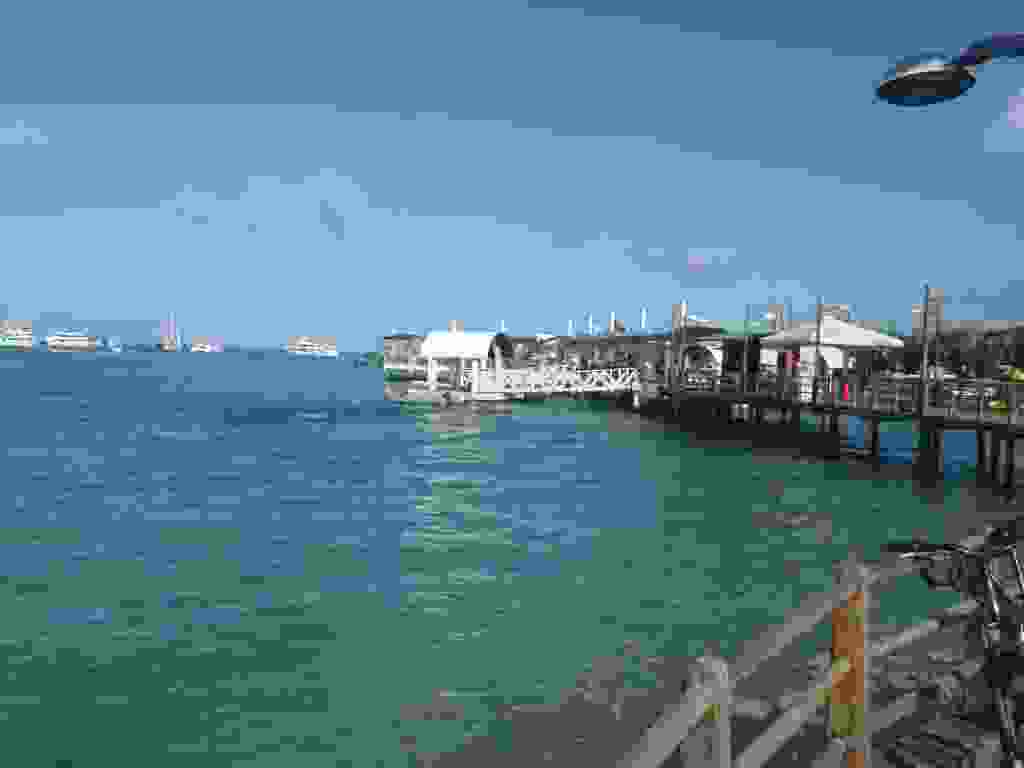
\includegraphics[width=\mywidth]{../wp-content/uploads/2015/07/P7015189-1024x768.jpg} } 
 \newline
 \newline
\centerline{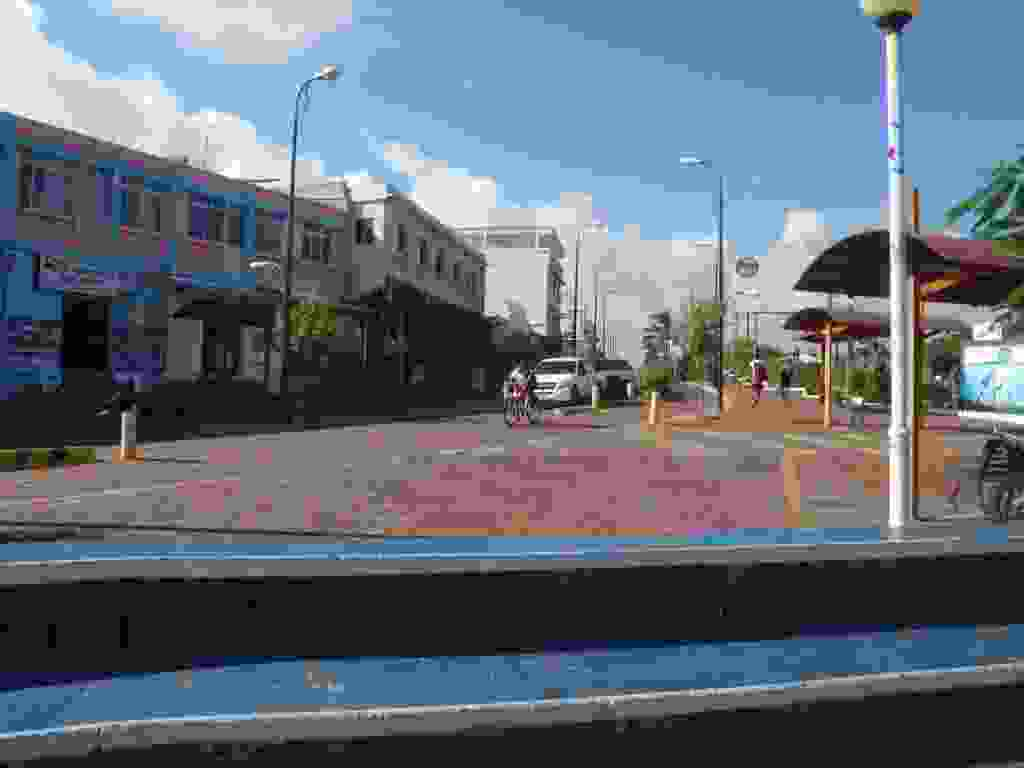
\includegraphics[width=\mywidth]{../wp-content/uploads/2015/07/P7015191-1024x768.jpg} } 
 \newline
 Je visite le centre Charles Darwin où on peut observer des tortues et des iguanes. \newline
 \newline
\centerline{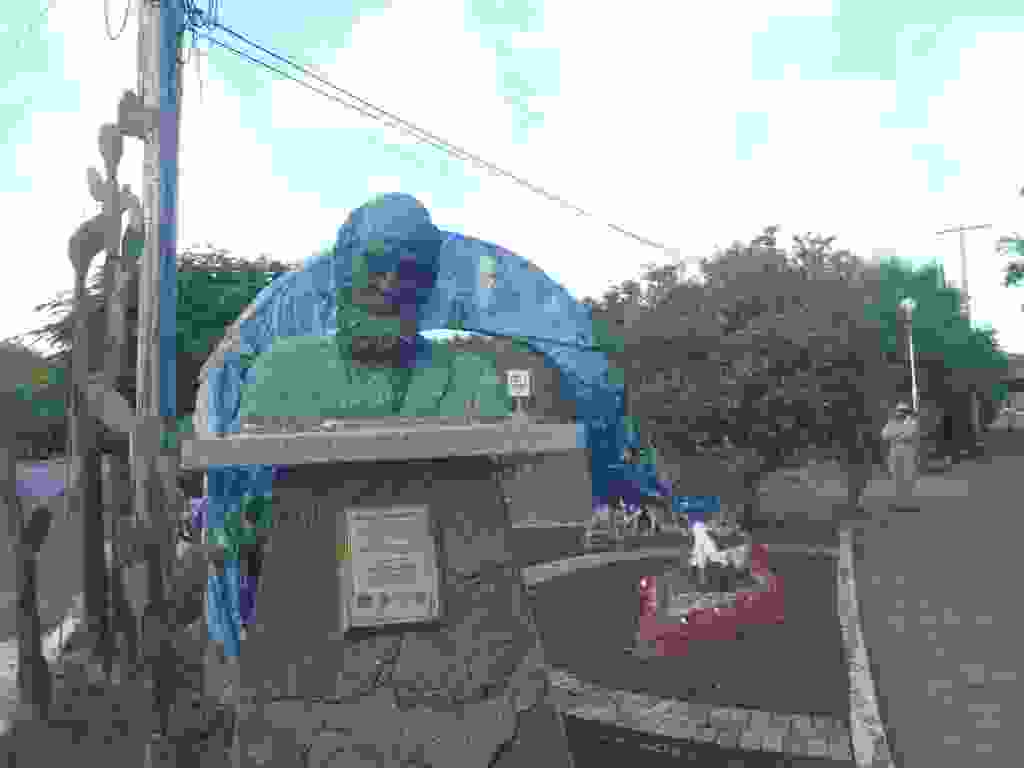
\includegraphics[width=\mywidth]{../wp-content/uploads/2015/07/P7025192-1024x768.jpg} } 
 \newline
 \newline
\centerline{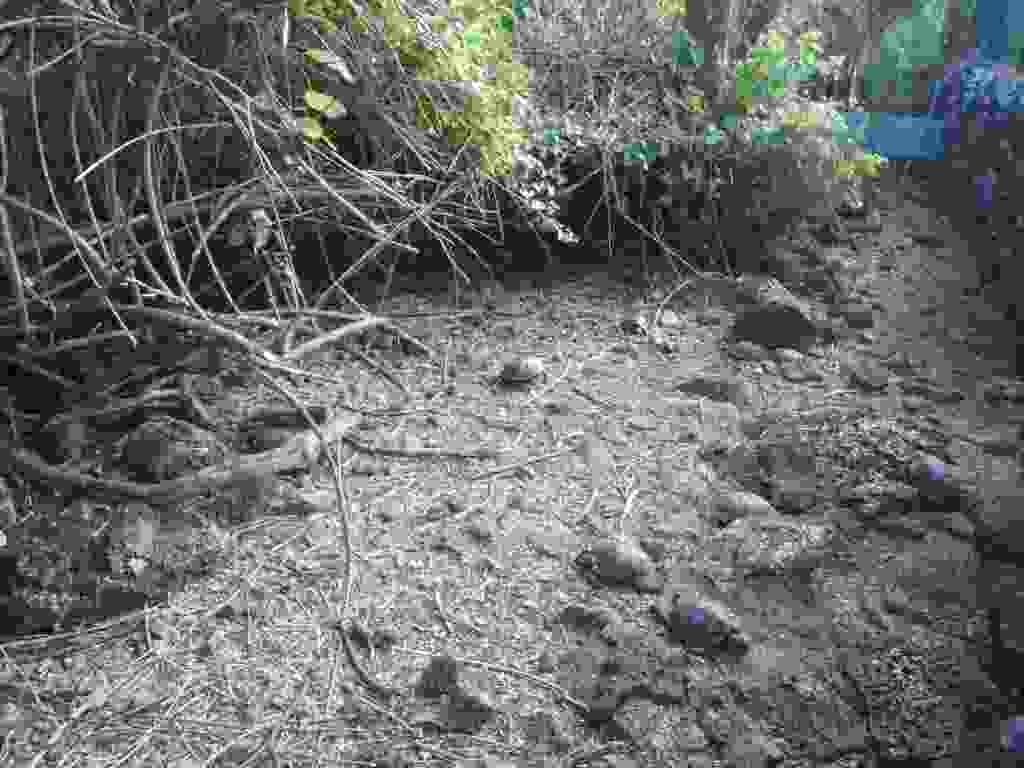
\includegraphics[width=\mywidth]{../wp-content/uploads/2015/07/P7025196-1024x768.jpg} } 
 \newline
 \newline
\centerline{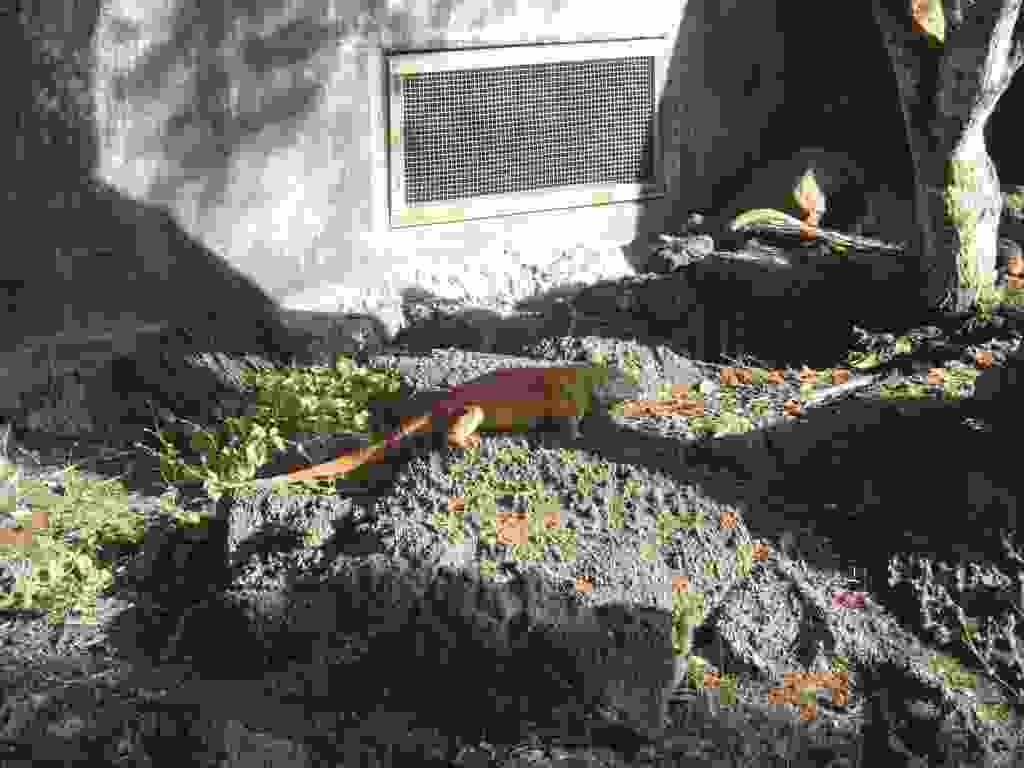
\includegraphics[width=\mywidth]{../wp-content/uploads/2015/07/P7025200-1024x768.jpg} } 
 \newline
 \newline
\centerline{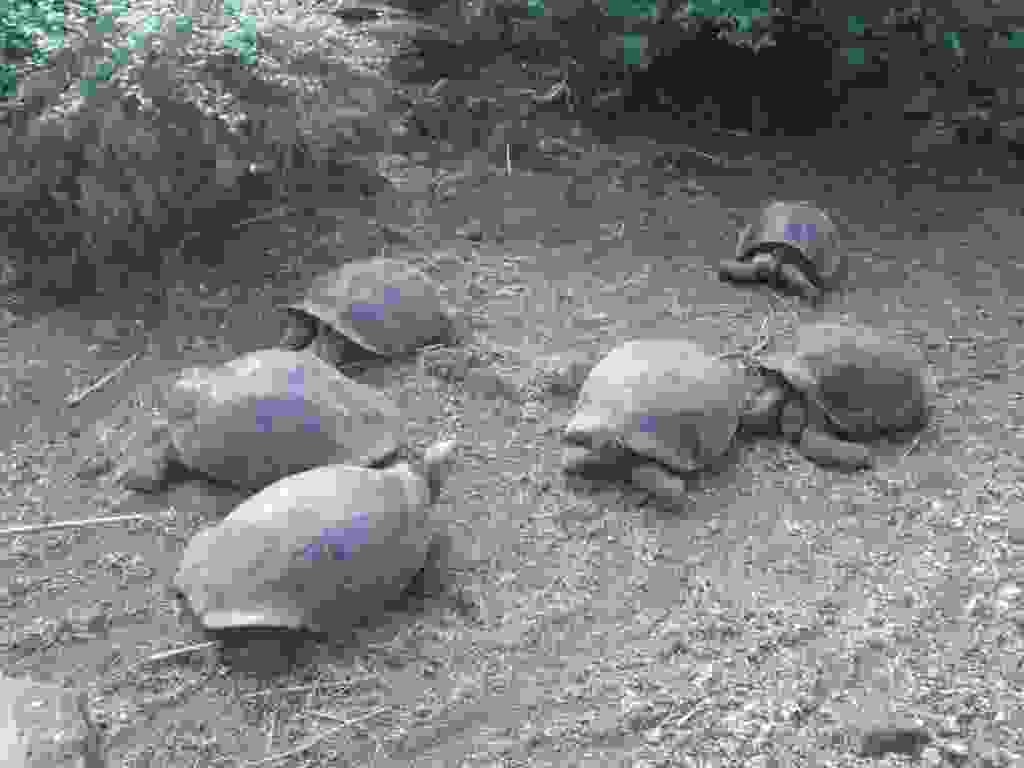
\includegraphics[width=\mywidth]{../wp-content/uploads/2015/07/P7025204-1024x768.jpg} } 
 \newline
 Je me rends en stop à la réserve d'El Chato au centre de l'île. Les tortues sont ici en liberté. \newline
 \newline
\centerline{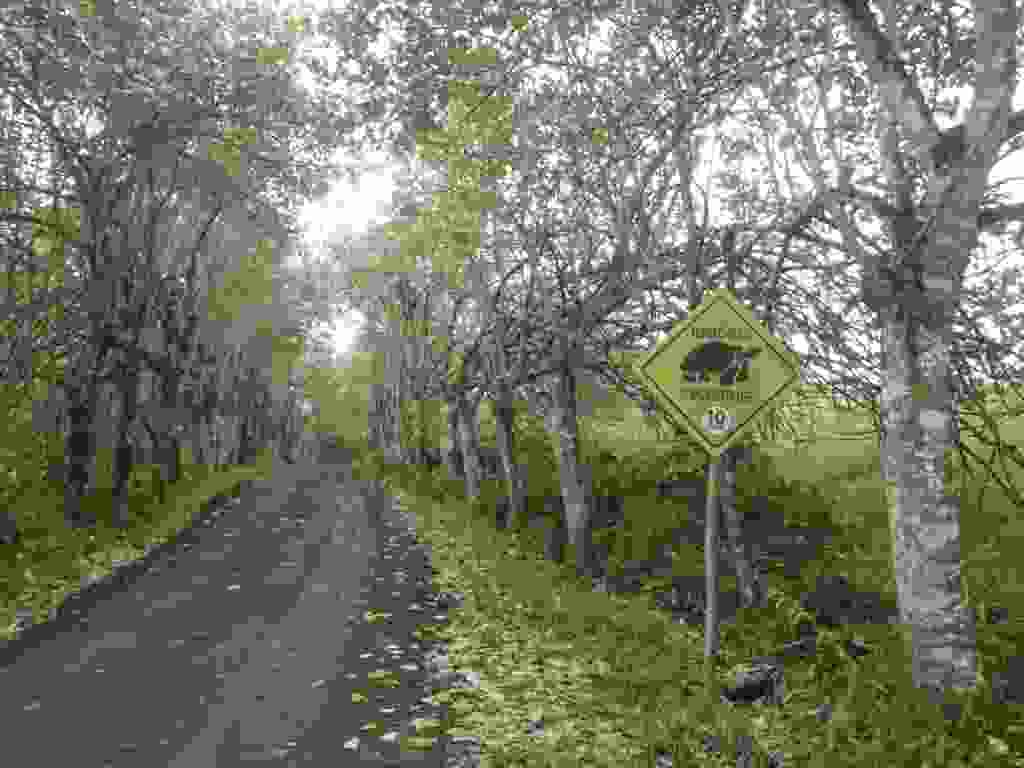
\includegraphics[width=\mywidth]{../wp-content/uploads/2015/07/P7025208-1024x768.jpg} } 
 \newline
 \newline
\centerline{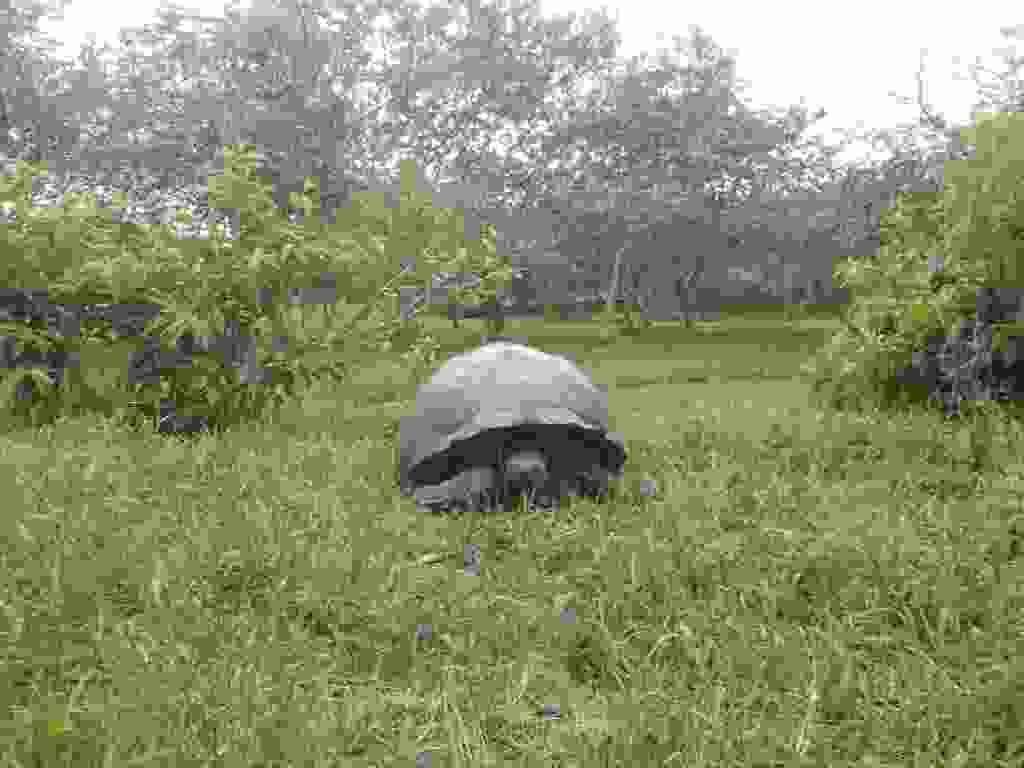
\includegraphics[width=\mywidth]{../wp-content/uploads/2015/07/P7025210-1024x768.jpg} } 
 \newline
 \newline
\centerline{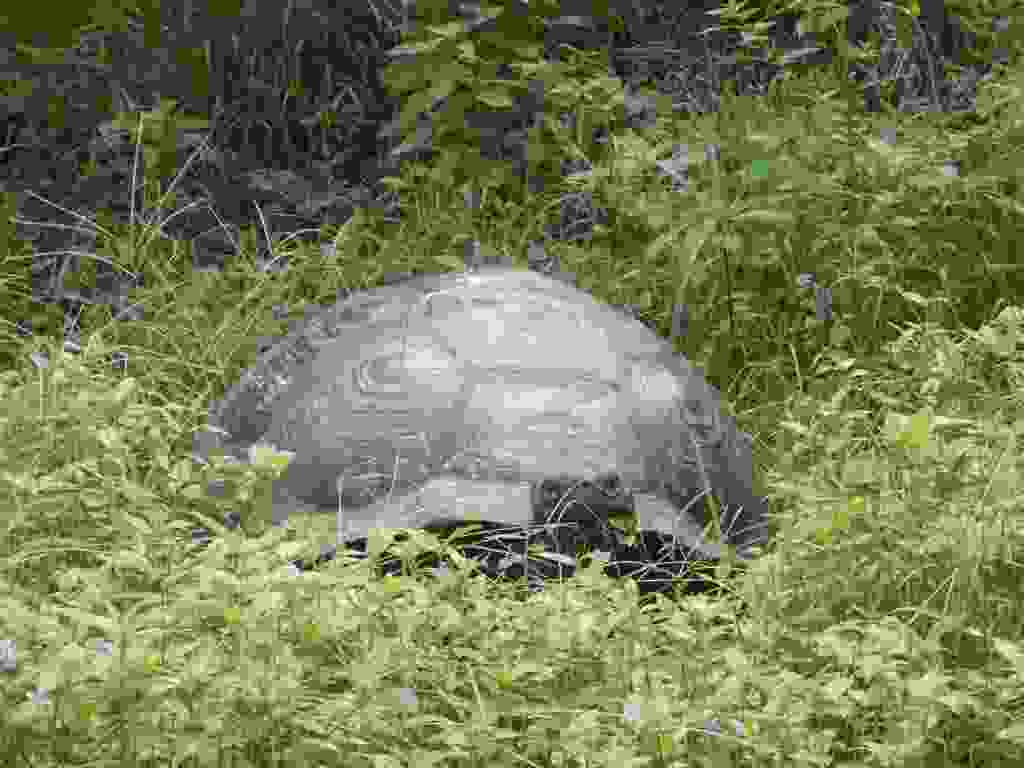
\includegraphics[width=\mywidth]{../wp-content/uploads/2015/07/P7025214-1024x768.jpg} } 
 \newline
 \newline
\centerline{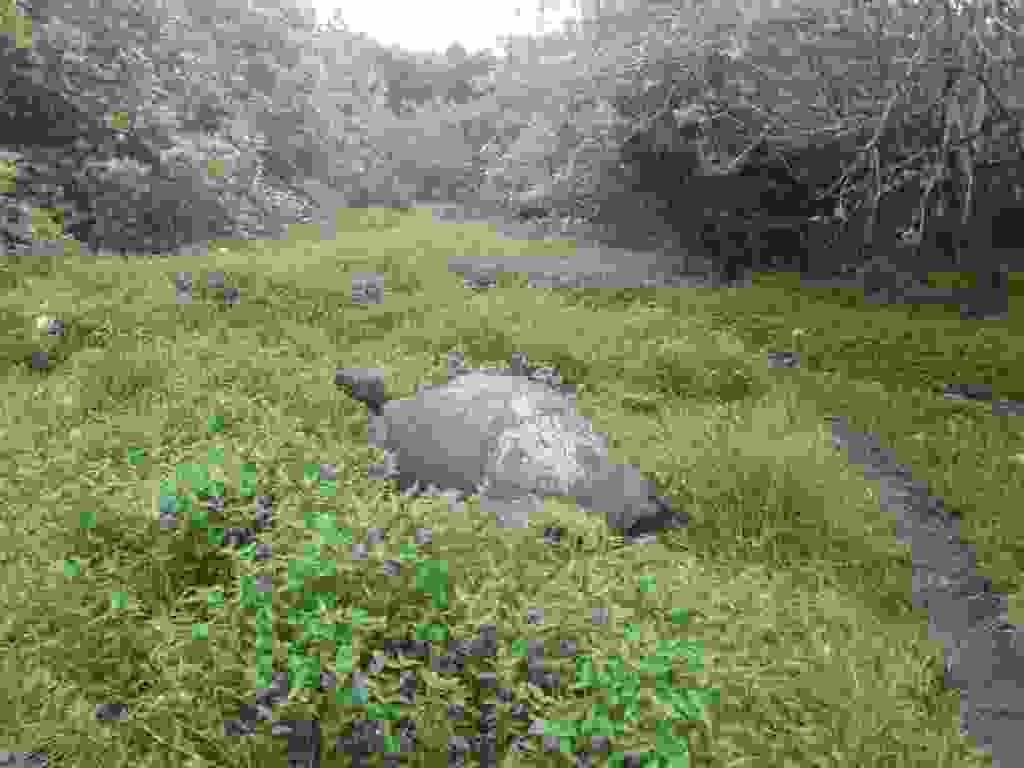
\includegraphics[width=\mywidth]{../wp-content/uploads/2015/07/P7025217-1024x768.jpg} } 
\newline
\centerline{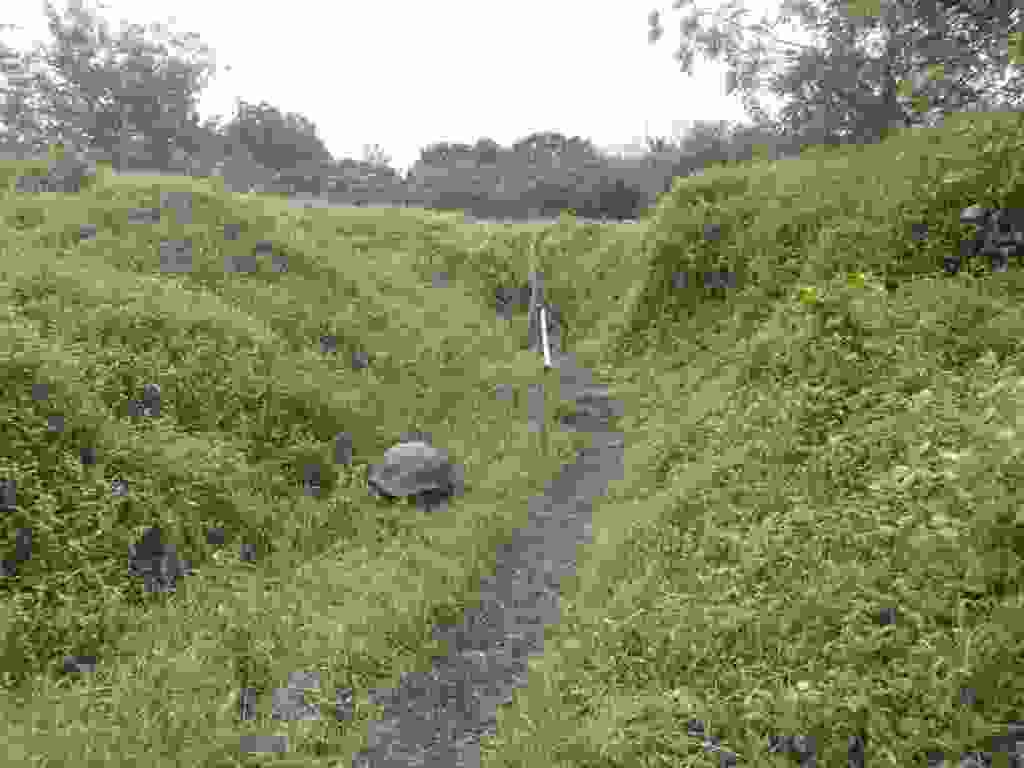
\includegraphics[width=\mywidth]{../wp-content/uploads/2015/07/P7025219-1024x768.jpg} } 
 \newline
 Il y aussi des tunnels de lave. \newline
 \newline
\centerline{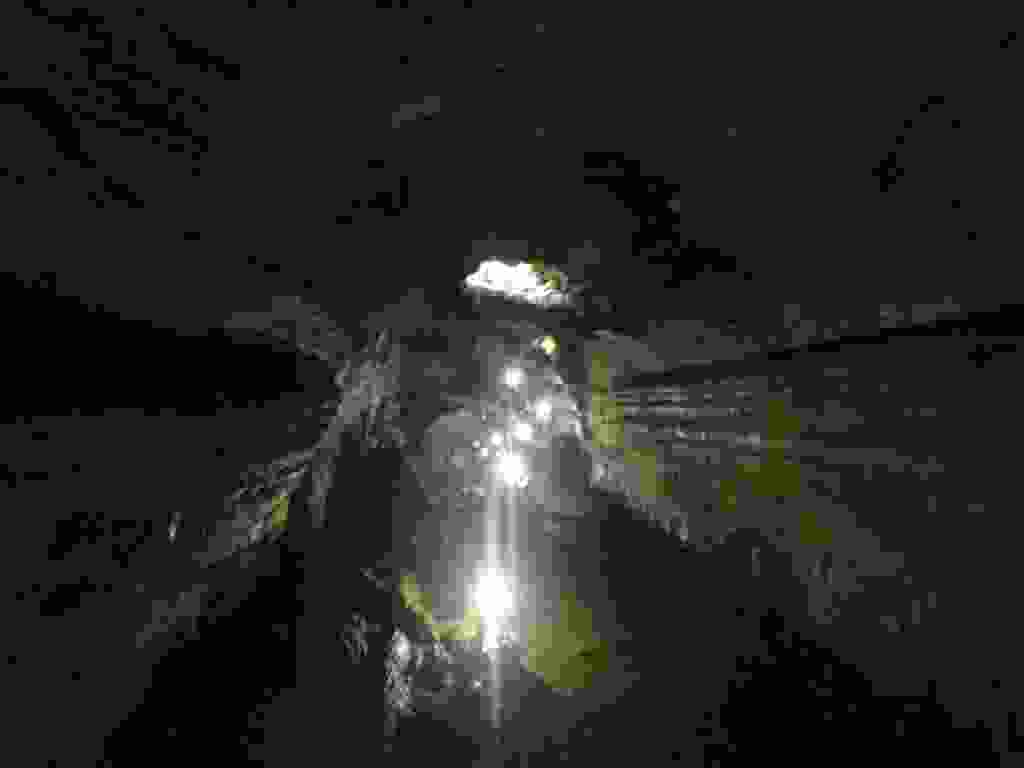
\includegraphics[width=\mywidth]{../wp-content/uploads/2015/07/P7025222-1024x768.jpg} } 
 \newline
 Jolie balade jusqu'au site de Las Grietas. \newline
 \newline
\centerline{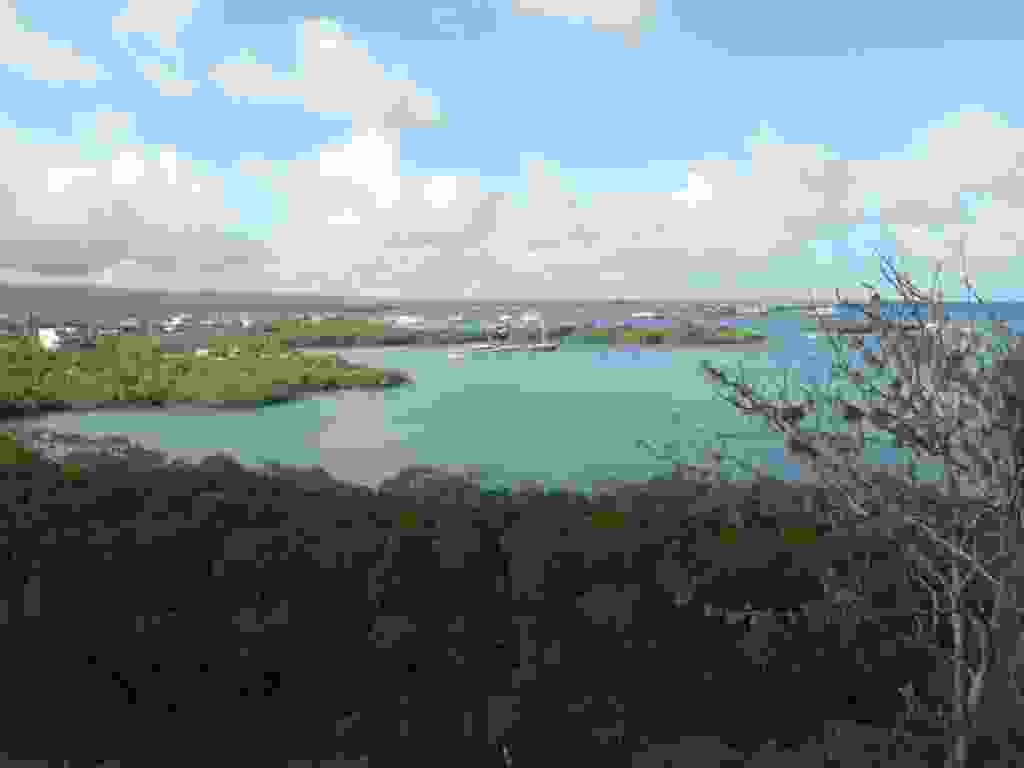
\includegraphics[width=\mywidth]{../wp-content/uploads/2015/07/P7035241-1024x768.jpg} } 
 \newline
 Petite plage, l'eau est bien chaude. \newline
 \newline
\centerline{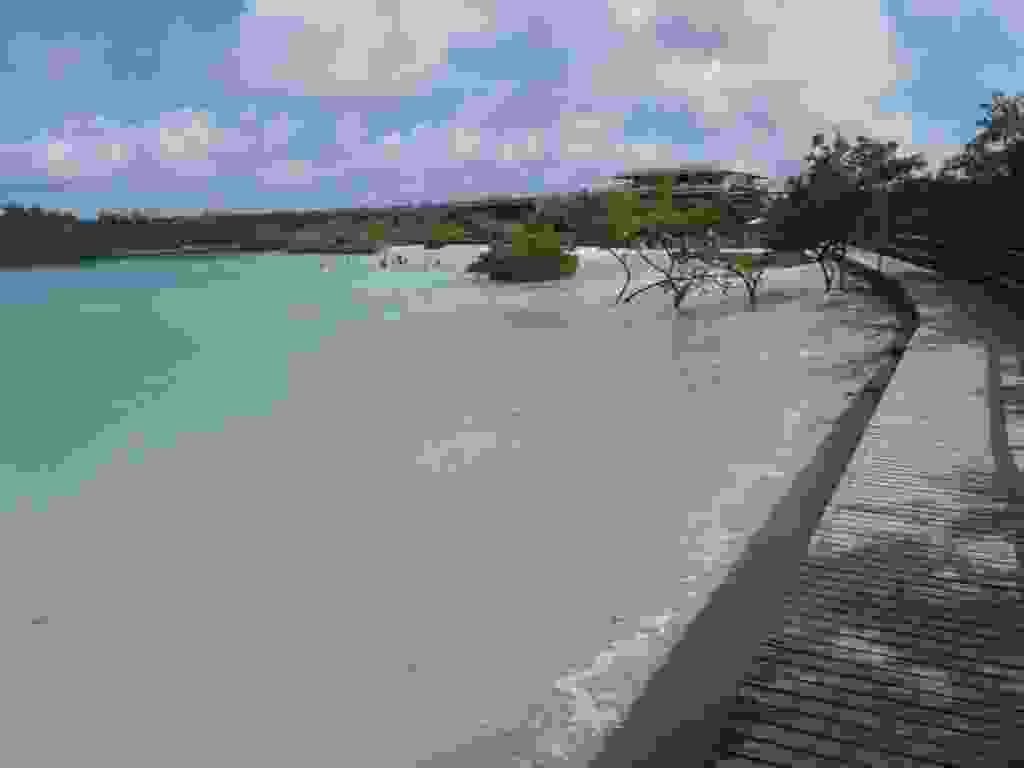
\includegraphics[width=\mywidth]{../wp-content/uploads/2015/07/P7025227-1024x768.jpg} } 
 \newline
 Snorkelling dans la faille, pas beaucoup de poissons mais l'endroit est agréable. \newline
 \newline
\centerline{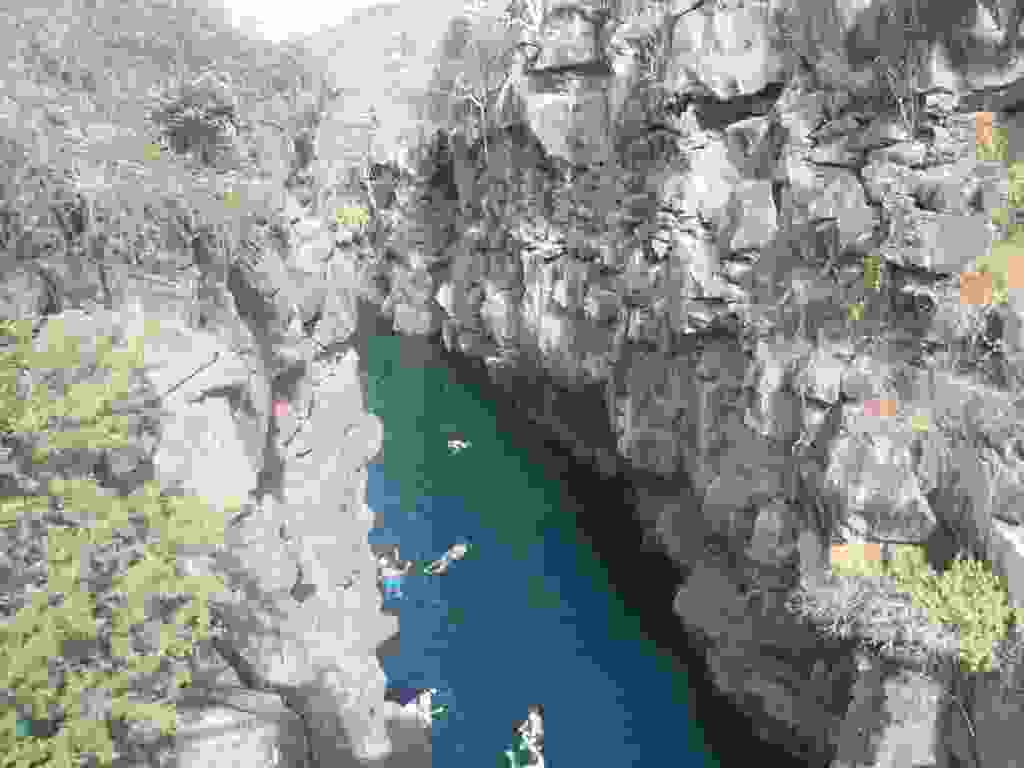
\includegraphics[width=\mywidth]{../wp-content/uploads/2015/07/P7025230-1024x768.jpg} } 
 \newline
 \newline
\centerline{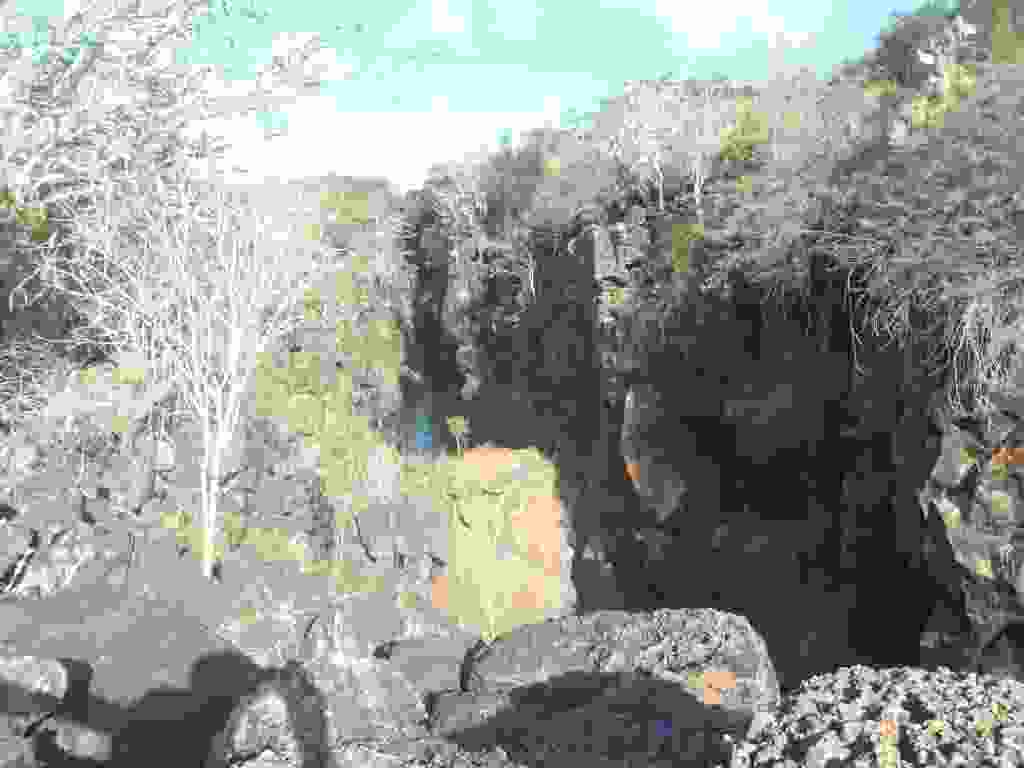
\includegraphics[width=\mywidth]{../wp-content/uploads/2015/07/P7035233-1024x768.jpg} } 
 \newline
 Le lendemain je passe la journée à Tortuga Bay à 1h de marche de Puerto Ayora. \newline
 \newline
\centerline{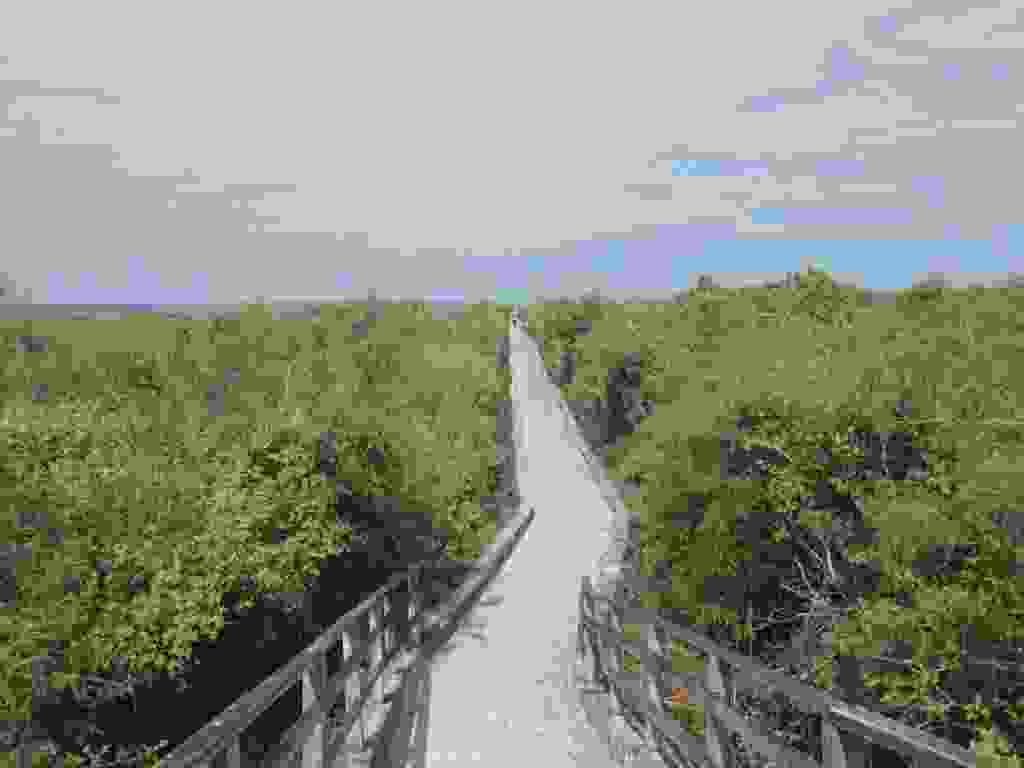
\includegraphics[width=\mywidth]{../wp-content/uploads/2015/07/P7035248-1024x768.jpg} } 
 \newline
 \newline
\centerline{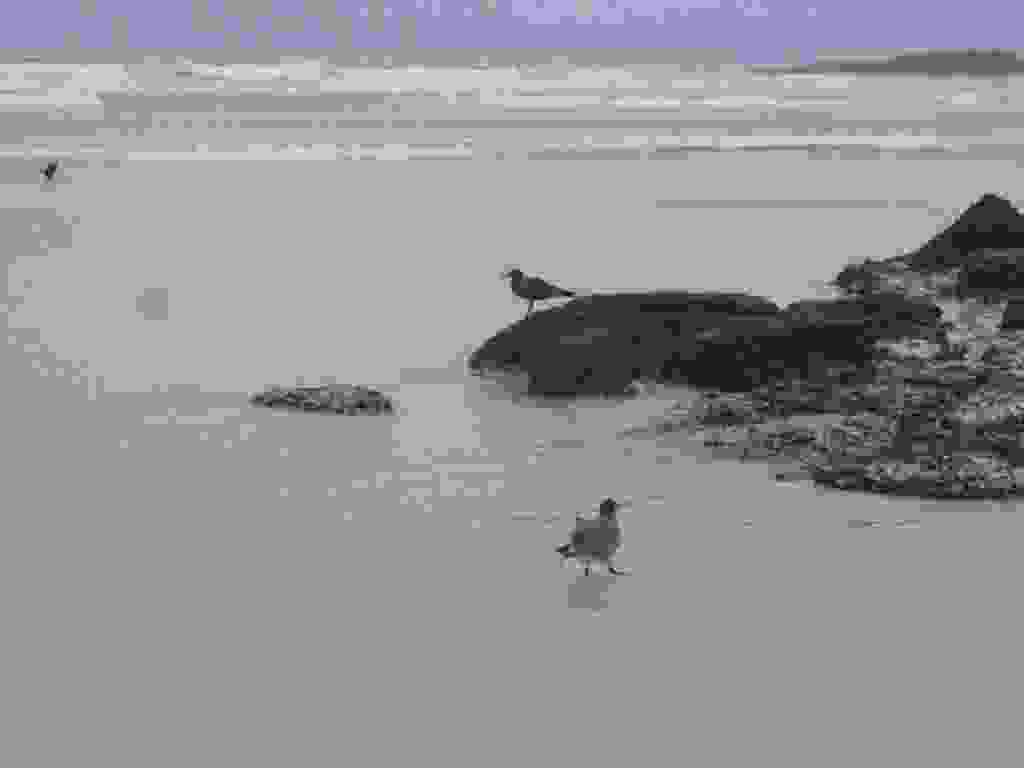
\includegraphics[width=\mywidth]{../wp-content/uploads/2015/07/P7035253-1024x768.jpg} } 
 \newline
 \newline
\centerline{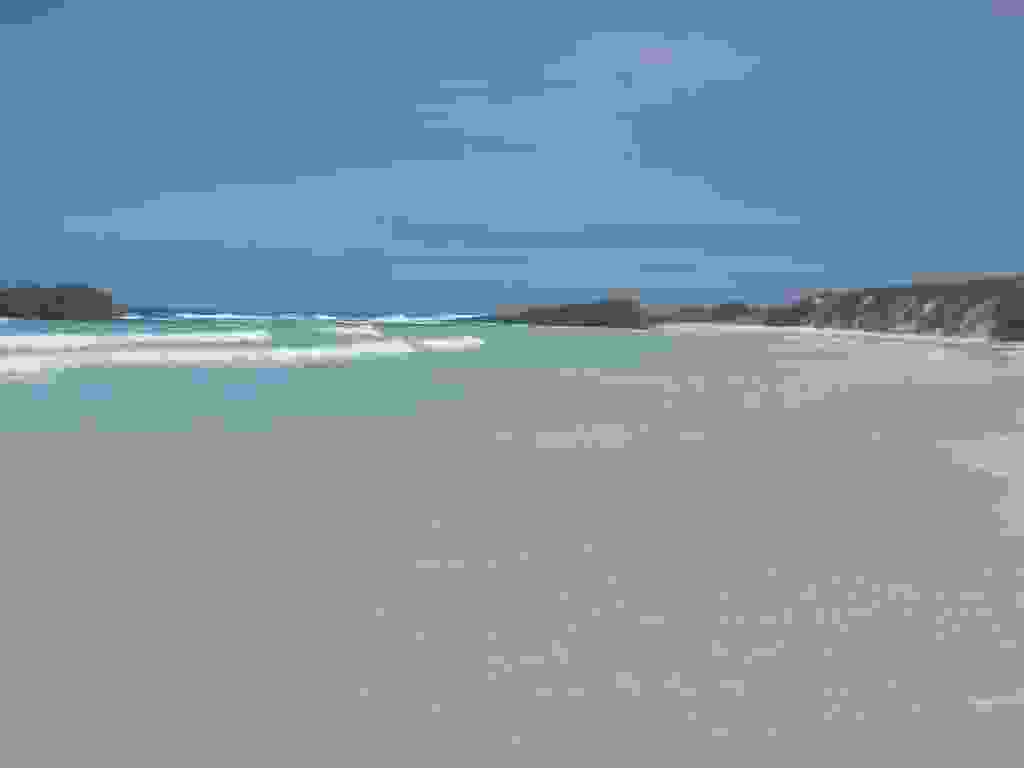
\includegraphics[width=\mywidth]{../wp-content/uploads/2015/07/P7035280-1024x768.jpg} } 
 \newline
 Beaucoup d'iguanes mais pas de tortues, en fait elle viennent sur la plage seulement pour déposer leurs oeufs. \newline
 \newline
\centerline{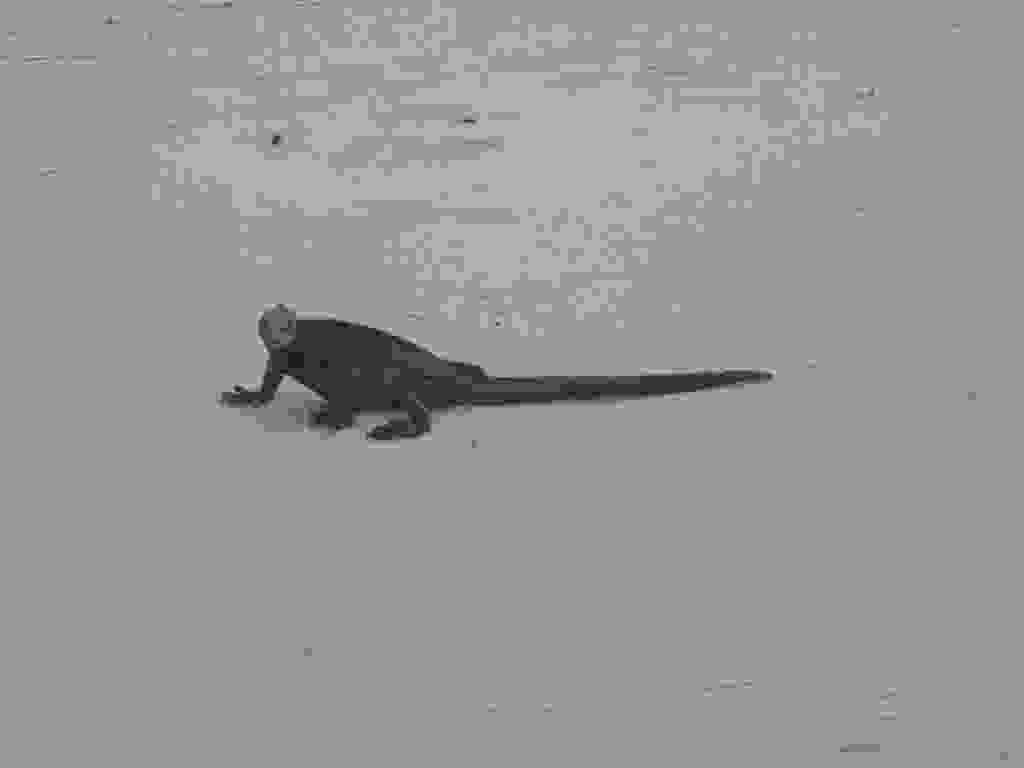
\includegraphics[width=\mywidth]{../wp-content/uploads/2015/07/P7035255-1024x768.jpg} } 
 \newline
 \newline
\centerline{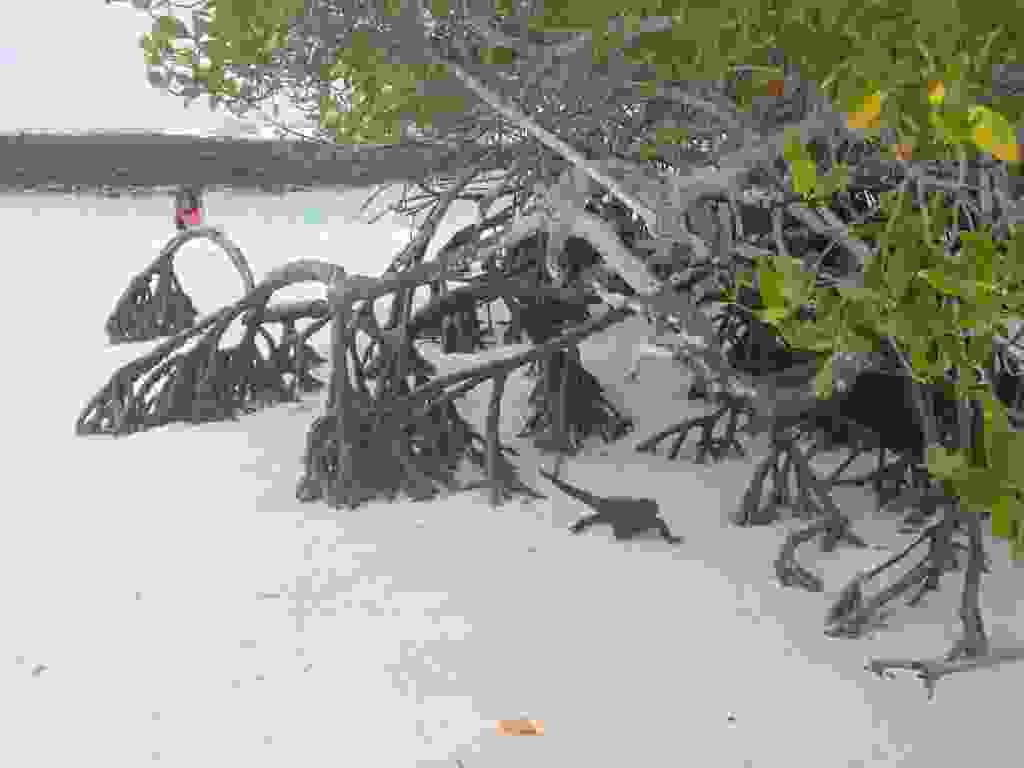
\includegraphics[width=\mywidth]{../wp-content/uploads/2015/07/P7035260-1024x768.jpg} } 
 \newline
 \newline
\centerline{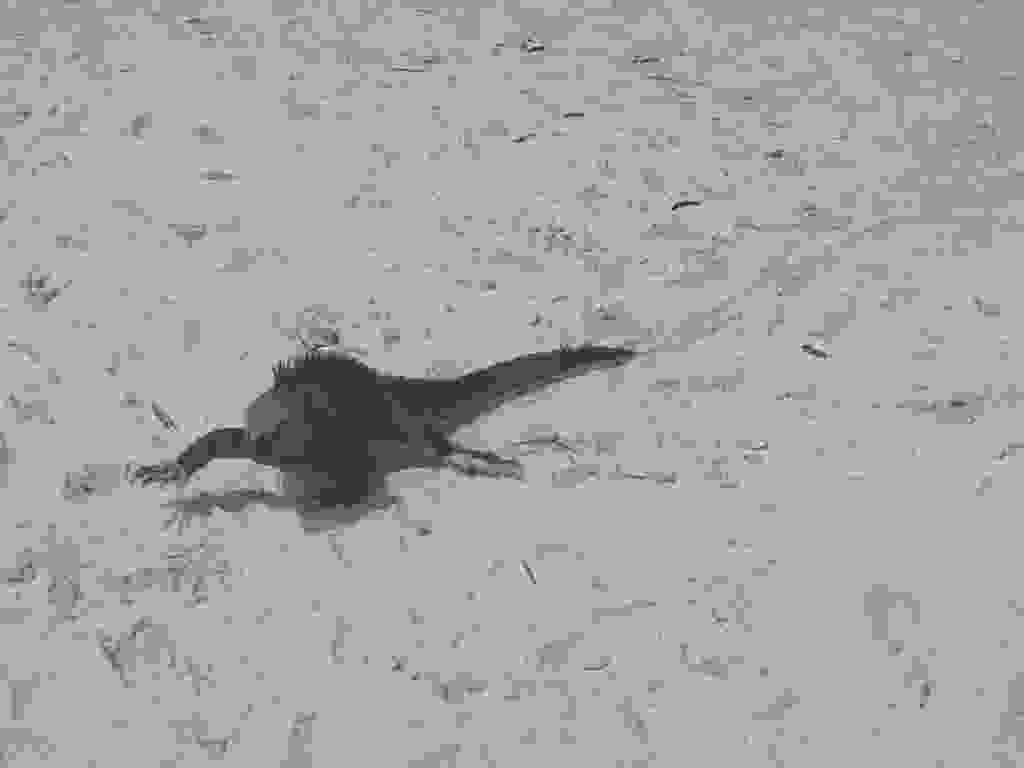
\includegraphics[width=\mywidth]{../wp-content/uploads/2015/07/P7035275-1024x768.jpg} } 
 \newline
 Je tente le snorkelling mais l'eau est bien trouble. \newline
 \newline
\centerline{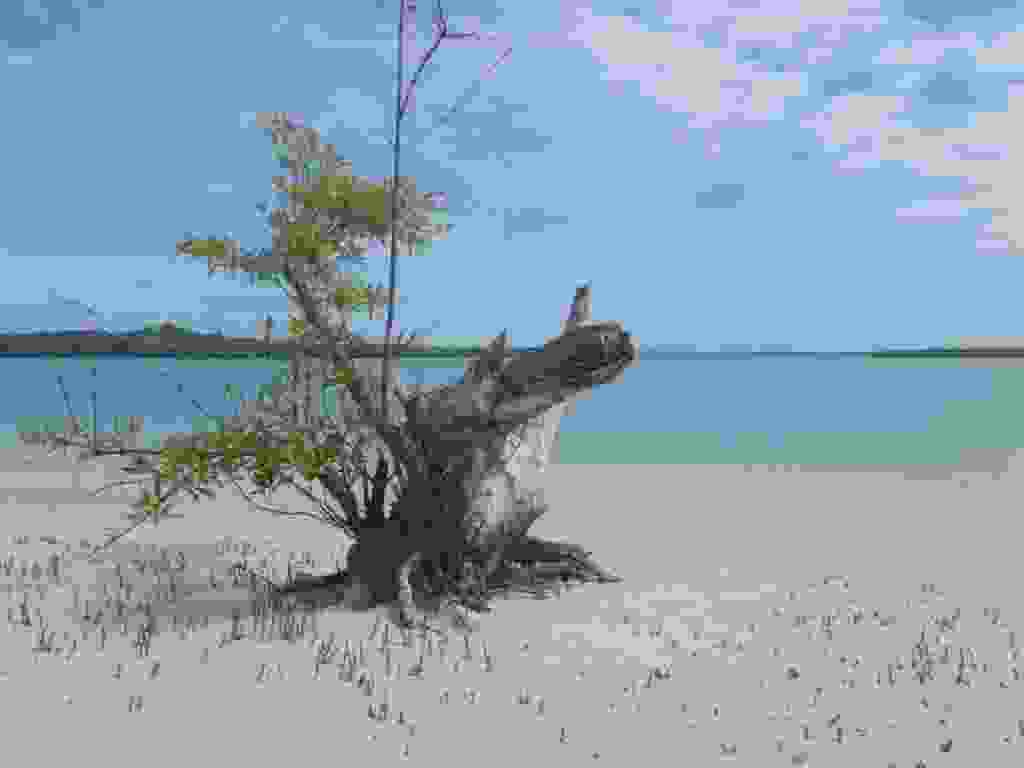
\includegraphics[width=\mywidth]{../wp-content/uploads/2015/07/P7035272-1024x768.jpg} } 
 \newline
 Après 3 jours sur l'île de Santa Cruz, je passe sur l'île d'Isabela qui est la plus grande des Galapagos. \newline
 \newline
\centerline{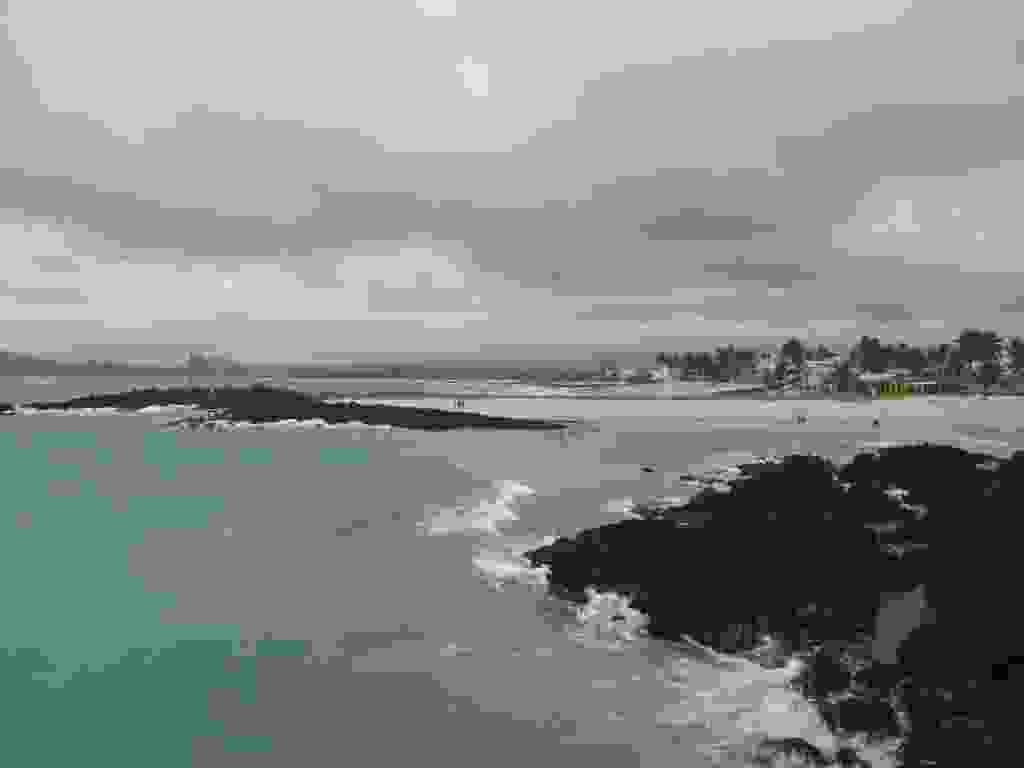
\includegraphics[width=\mywidth]{../wp-content/uploads/2015/07/P7045281-1024x768.jpg} } 
 \newline
 \newline
\centerline{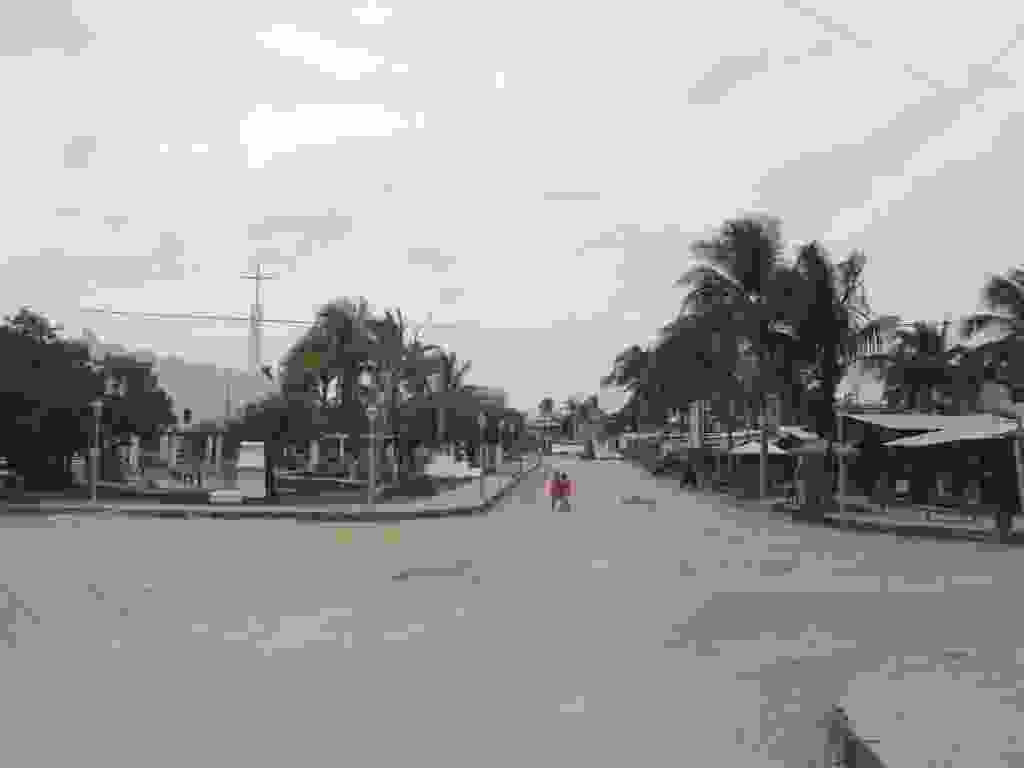
\includegraphics[width=\mywidth]{../wp-content/uploads/2015/07/P7045285-1024x768.jpg} } 
 \newline
 5km à pied pour voir le mur des larmes construit par des prisonniers à l'époque où l'île servait de bagne. \newline
 \newline
\centerline{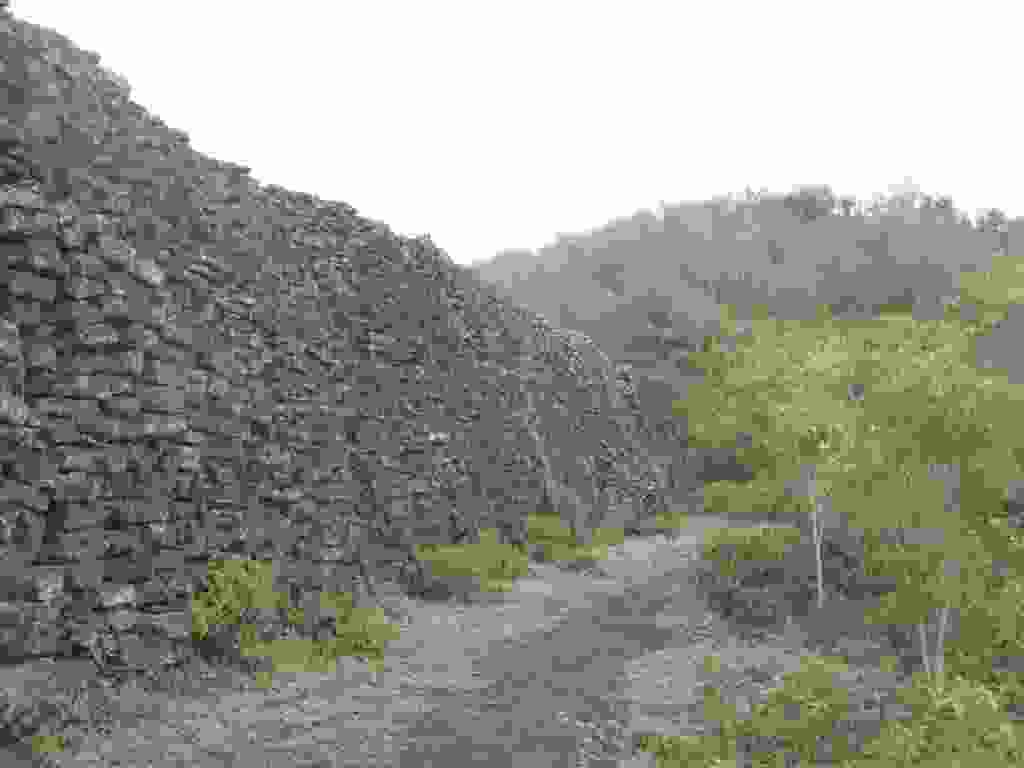
\includegraphics[width=\mywidth]{../wp-content/uploads/2015/07/P7045317-1024x768.jpg} } 
 \newline
 En chemin, des belles plages et des dizaines d'iguanes. \newline
 \newline
\centerline{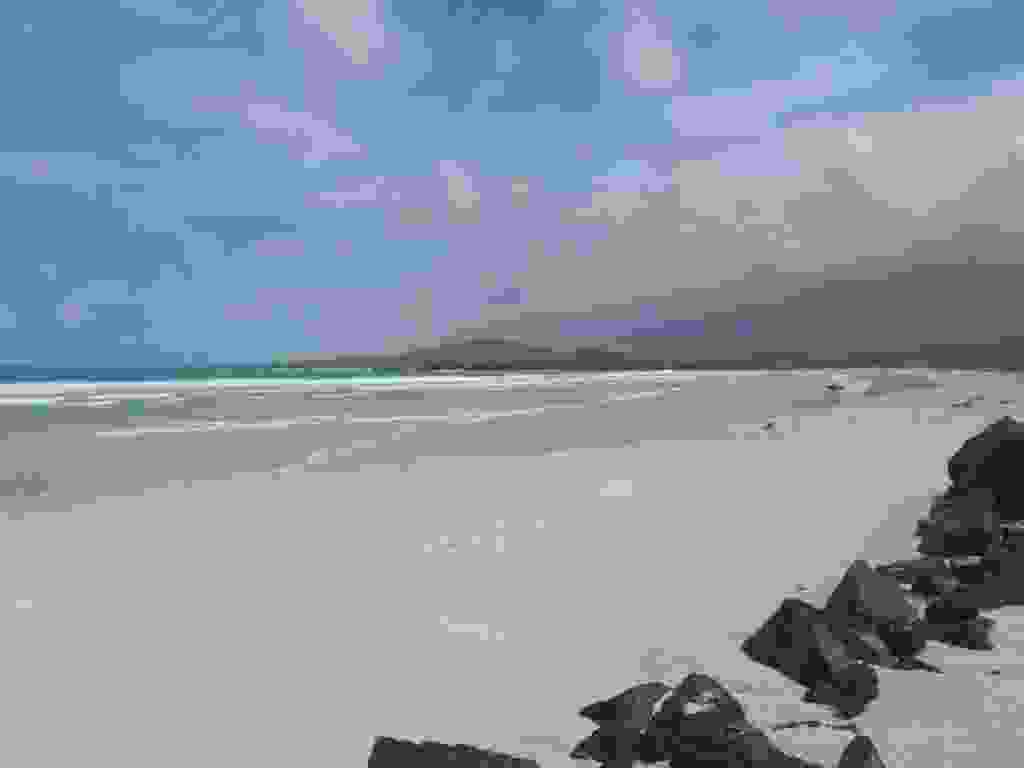
\includegraphics[width=\mywidth]{../wp-content/uploads/2015/07/P7045289-1024x768.jpg} } 
 \newline
 \newline
\centerline{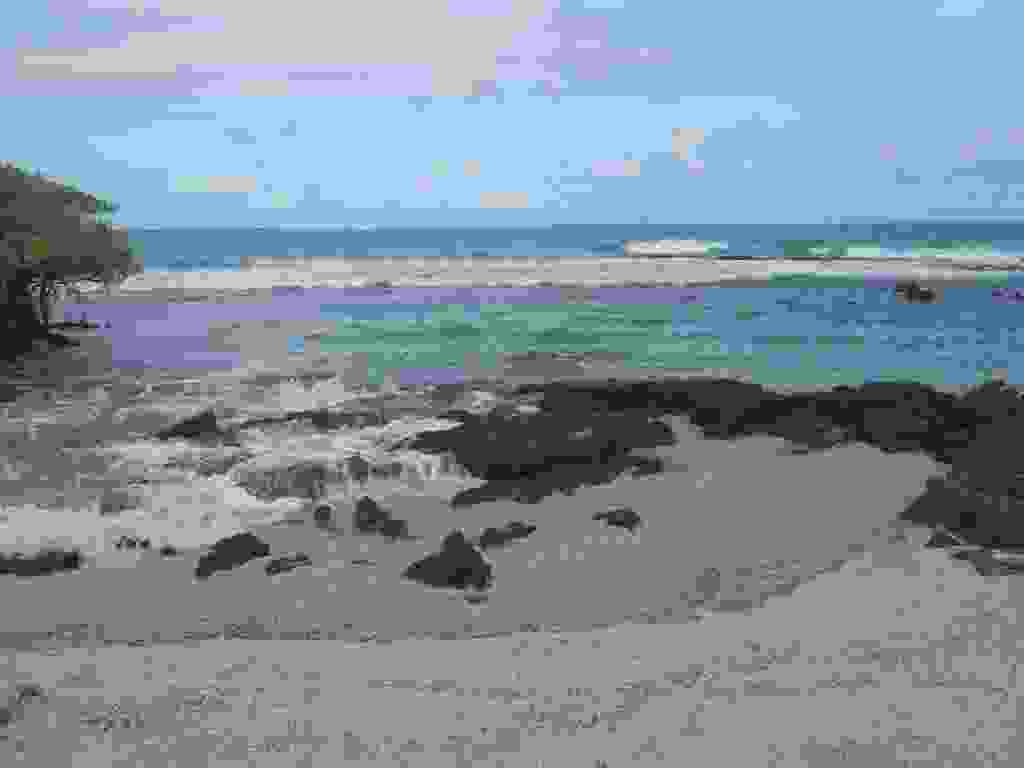
\includegraphics[width=\mywidth]{../wp-content/uploads/2015/07/P7045324-1024x768.jpg} } 
 \newline
 \newline
\centerline{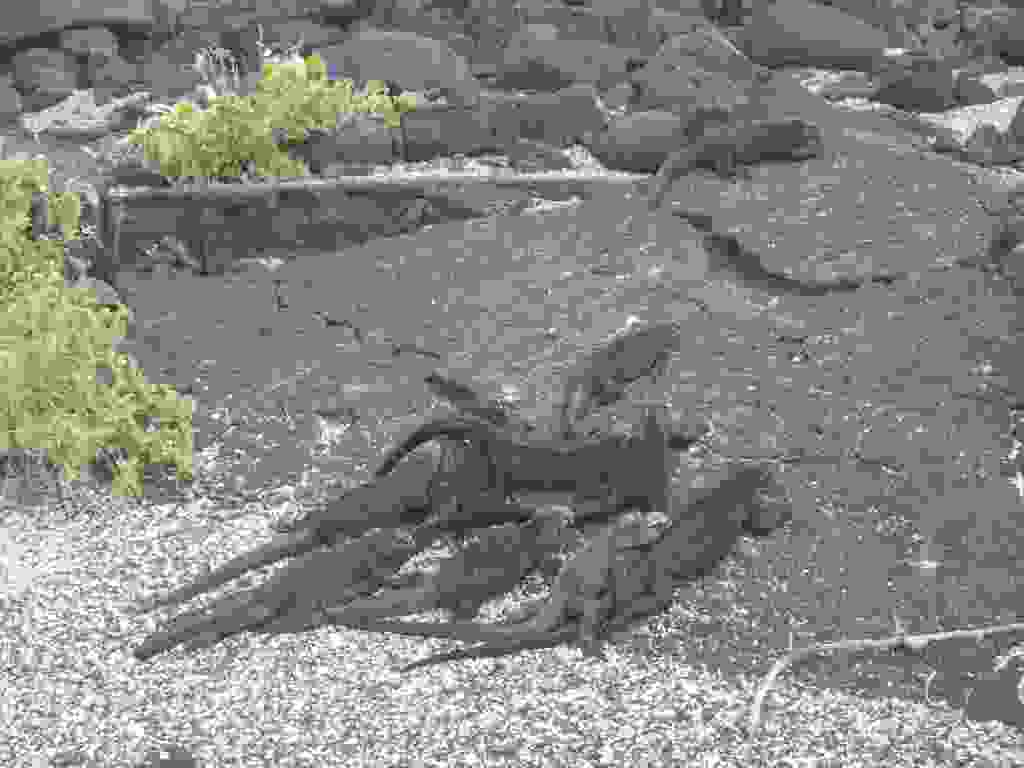
\includegraphics[width=\mywidth]{../wp-content/uploads/2015/07/P7045326-1024x768.jpg} } 
 \newline
 \newline
\centerline{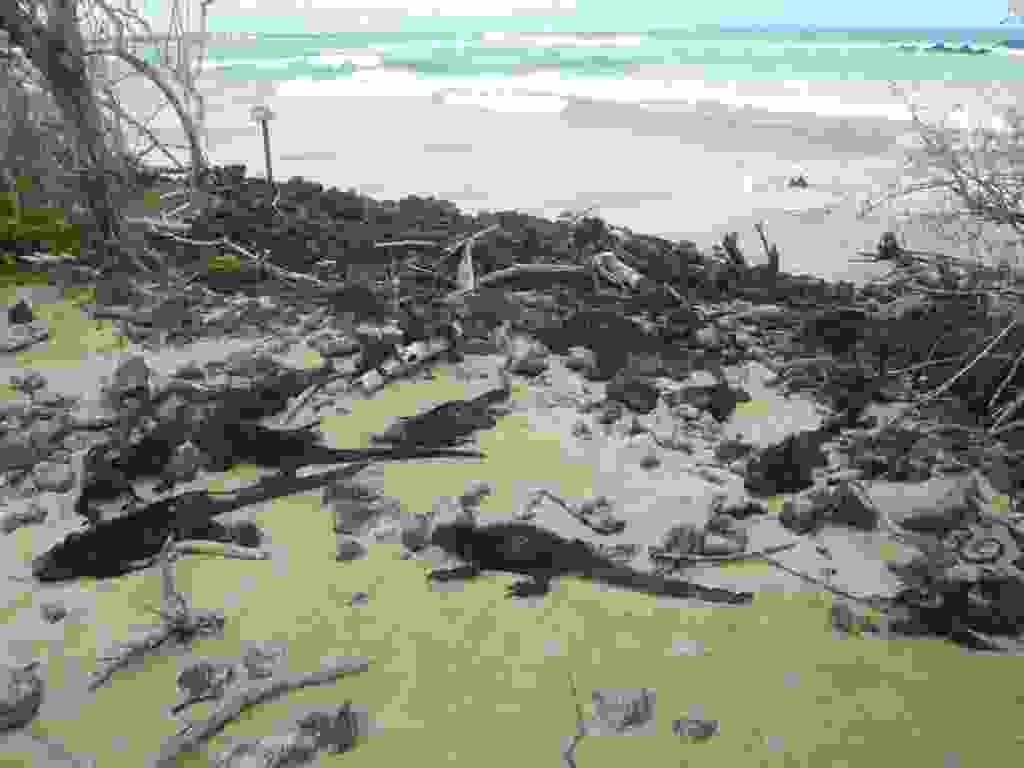
\includegraphics[width=\mywidth]{../wp-content/uploads/2015/07/P7045330-1024x768.jpg} } 
 \newline
 \newline
\centerline{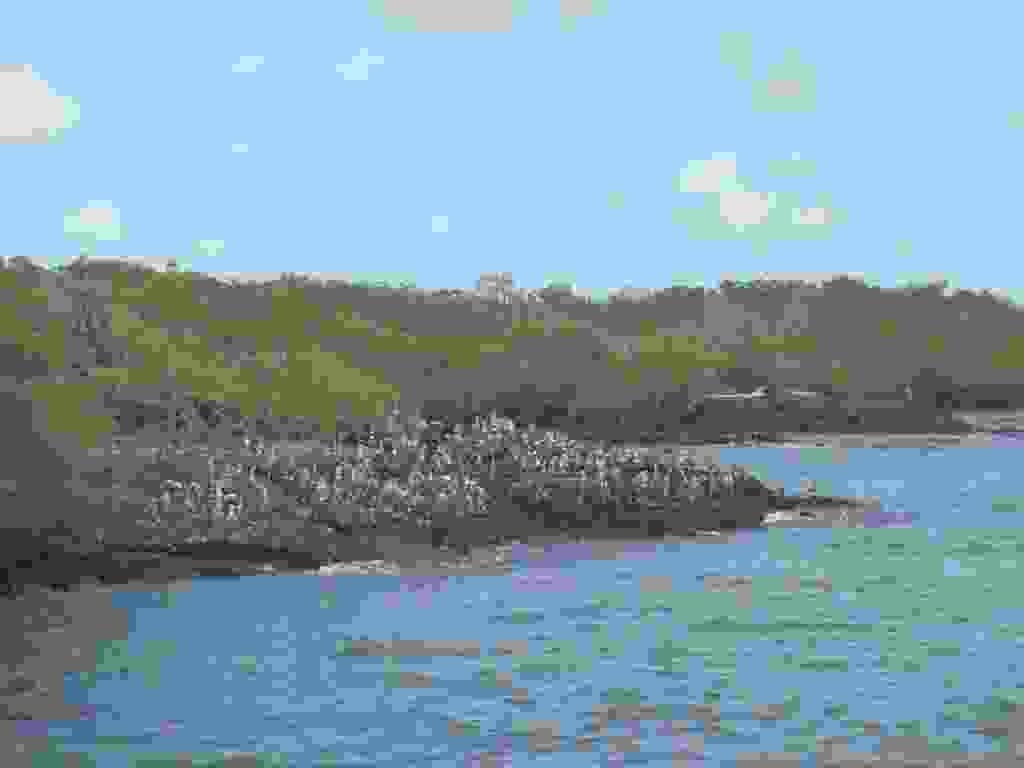
\includegraphics[width=\mywidth]{../wp-content/uploads/2015/07/P7045299-1024x768.jpg} } 
 \newline
 Quelques tortues. \newline
 \newline
\centerline{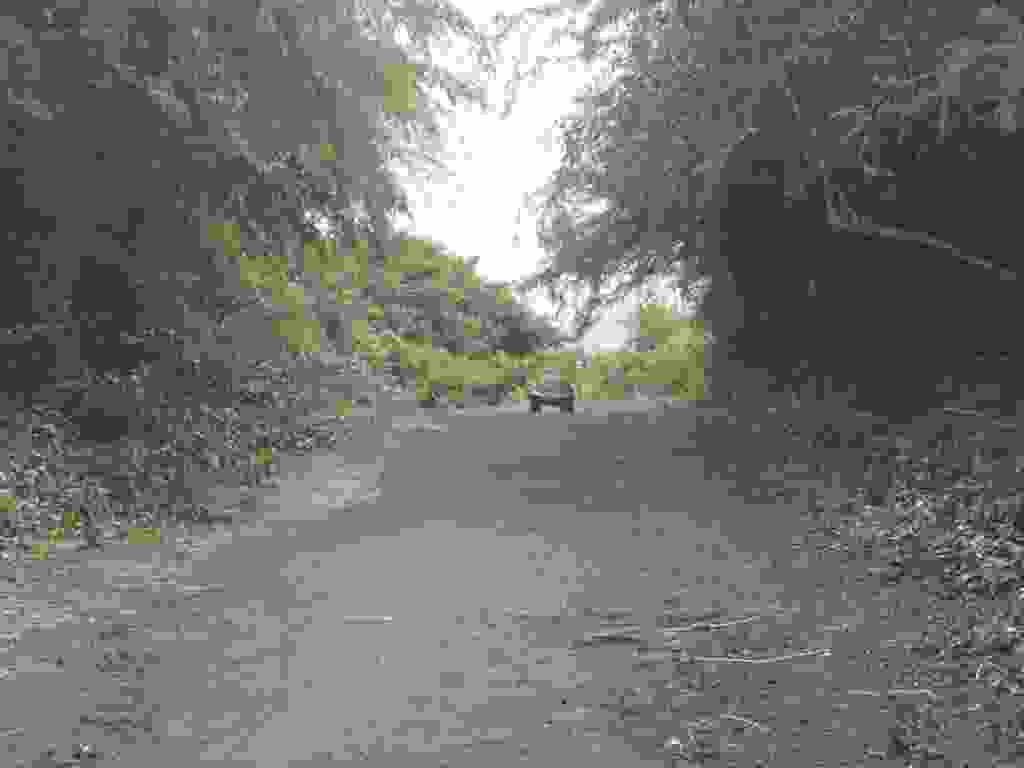
\includegraphics[width=\mywidth]{../wp-content/uploads/2015/07/P7045305-1024x768.jpg} } 
 \newline
 \newline
\centerline{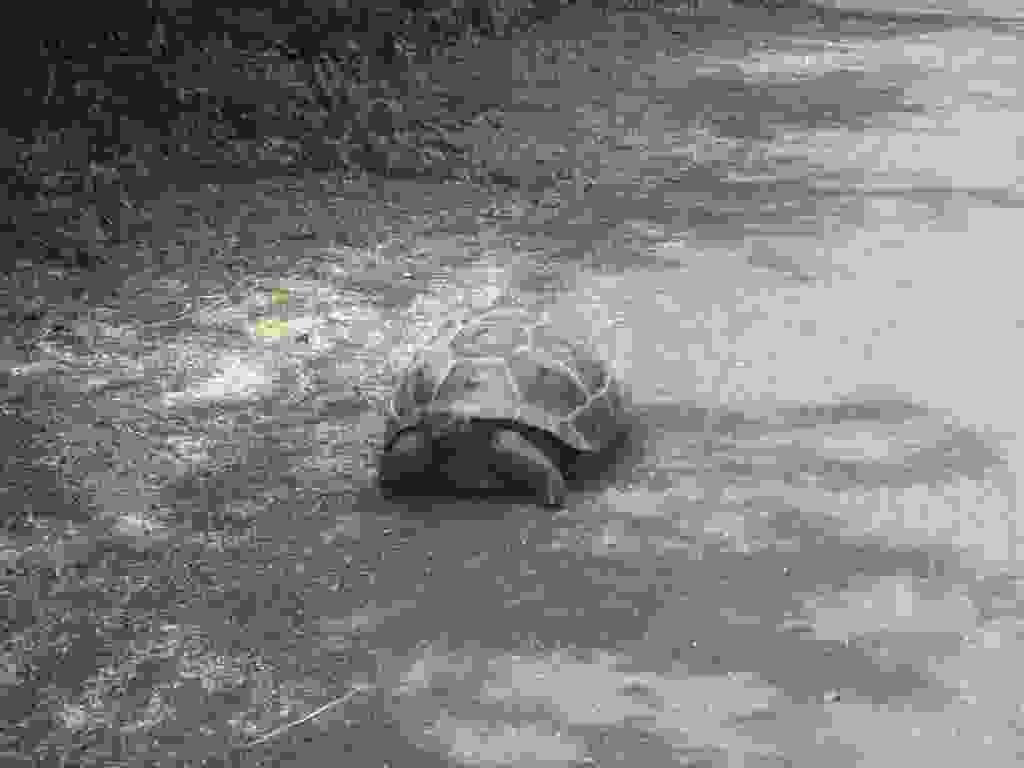
\includegraphics[width=\mywidth]{../wp-content/uploads/2015/07/P7045309-1024x768.jpg} } 
 \newline
 \newline
\centerline{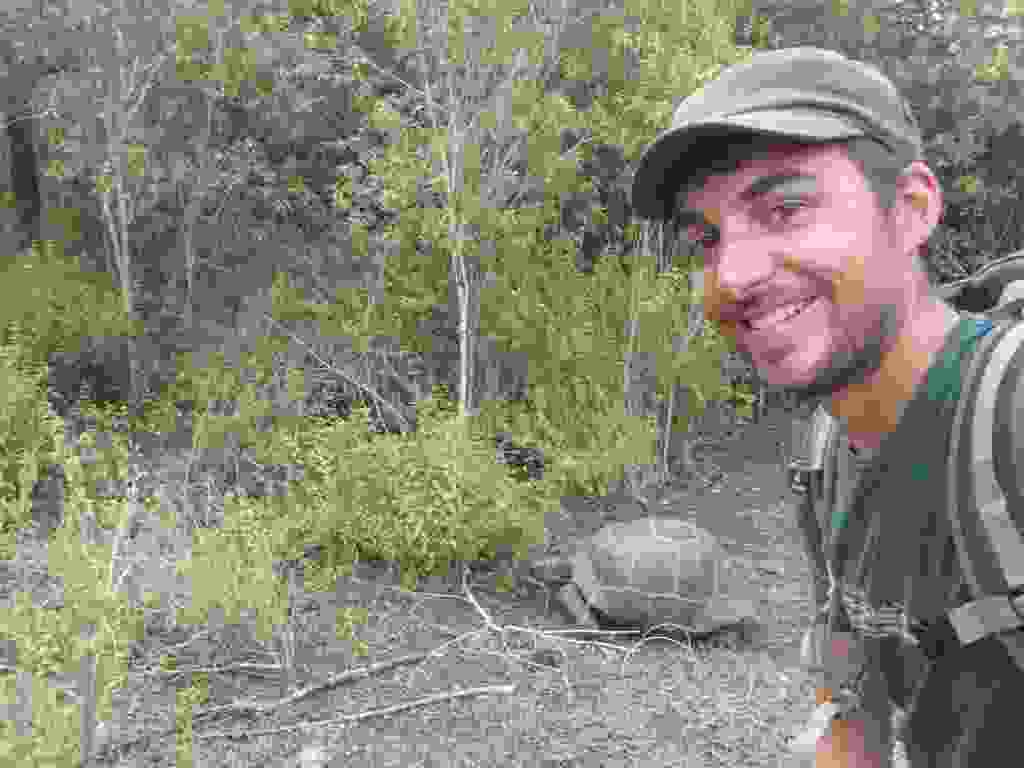
\includegraphics[width=\mywidth]{../wp-content/uploads/2015/07/P7045321-1024x768.jpg} } 
 \newline
 Le chemin traverse une zone humide de l'île, avec la mangrove. \newline
 \newline
\centerline{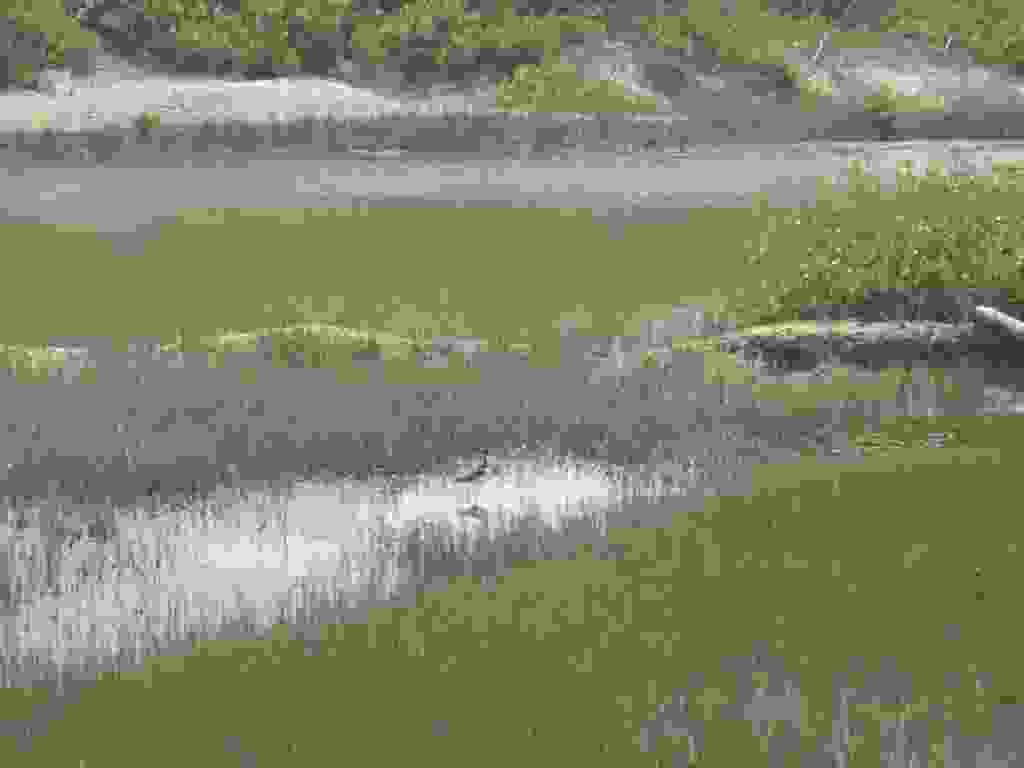
\includegraphics[width=\mywidth]{../wp-content/uploads/2015/07/P7045290-1024x768.jpg} } 
 \newline
 \newline
\centerline{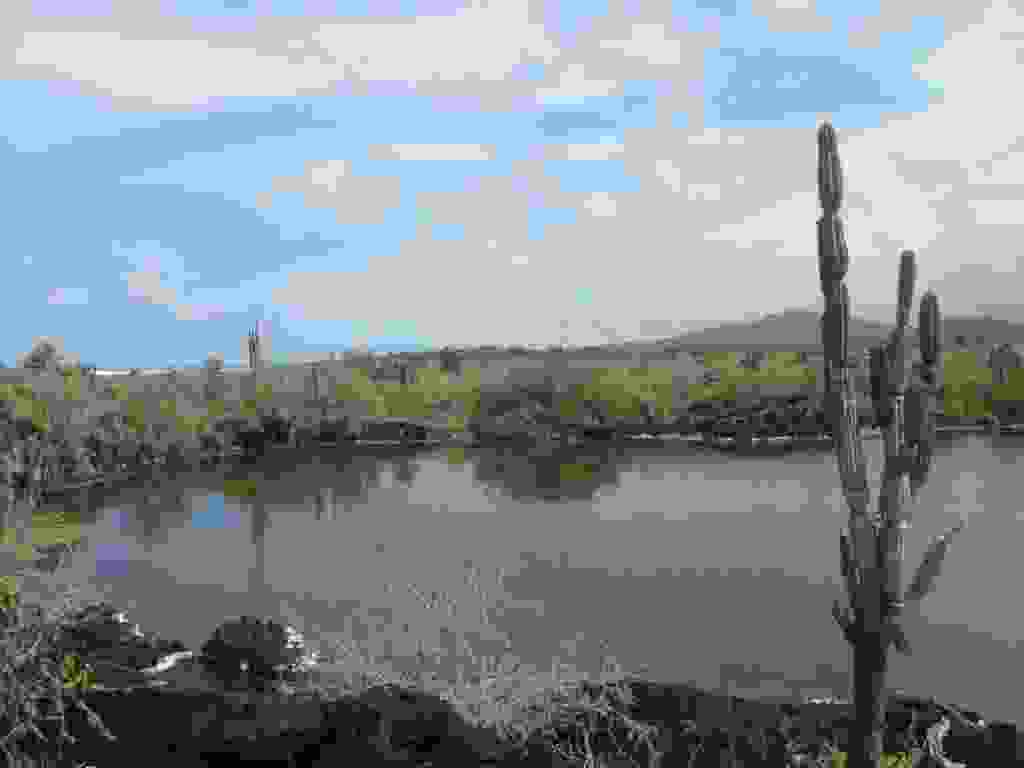
\includegraphics[width=\mywidth]{../wp-content/uploads/2015/07/P7045293-1024x768.jpg} } 
 \newline
 \newline
\centerline{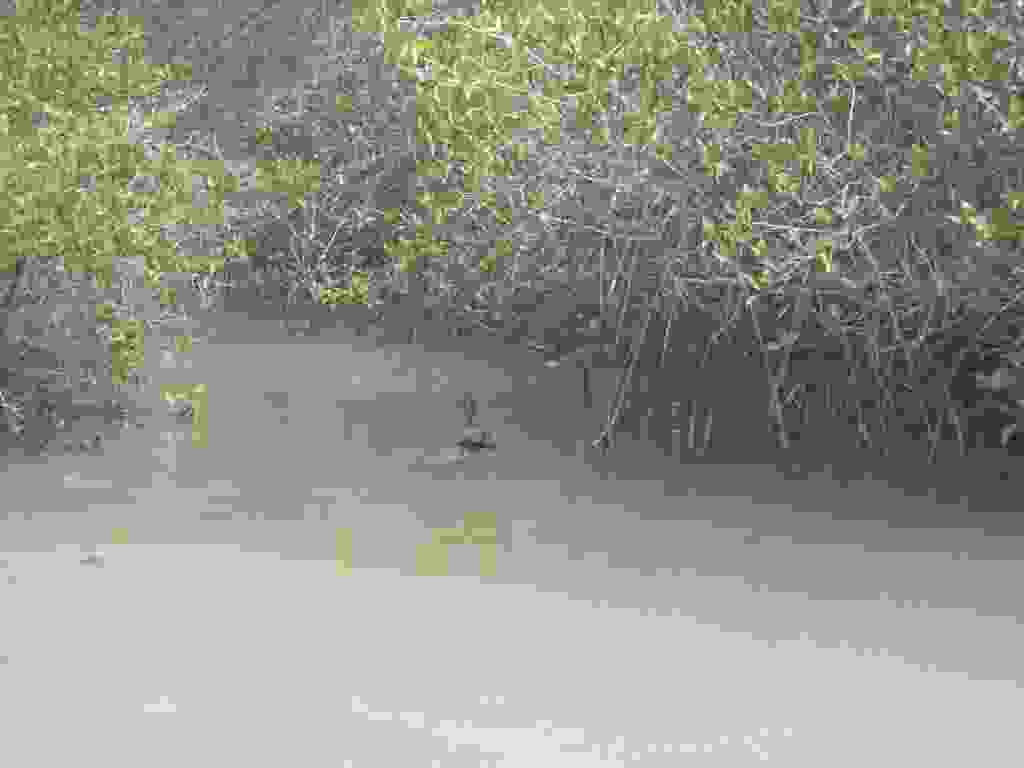
\includegraphics[width=\mywidth]{../wp-content/uploads/2015/07/P7045304-1024x768.jpg} } 
 \newline
 Un tunnel de lave. \newline
 \newline
\centerline{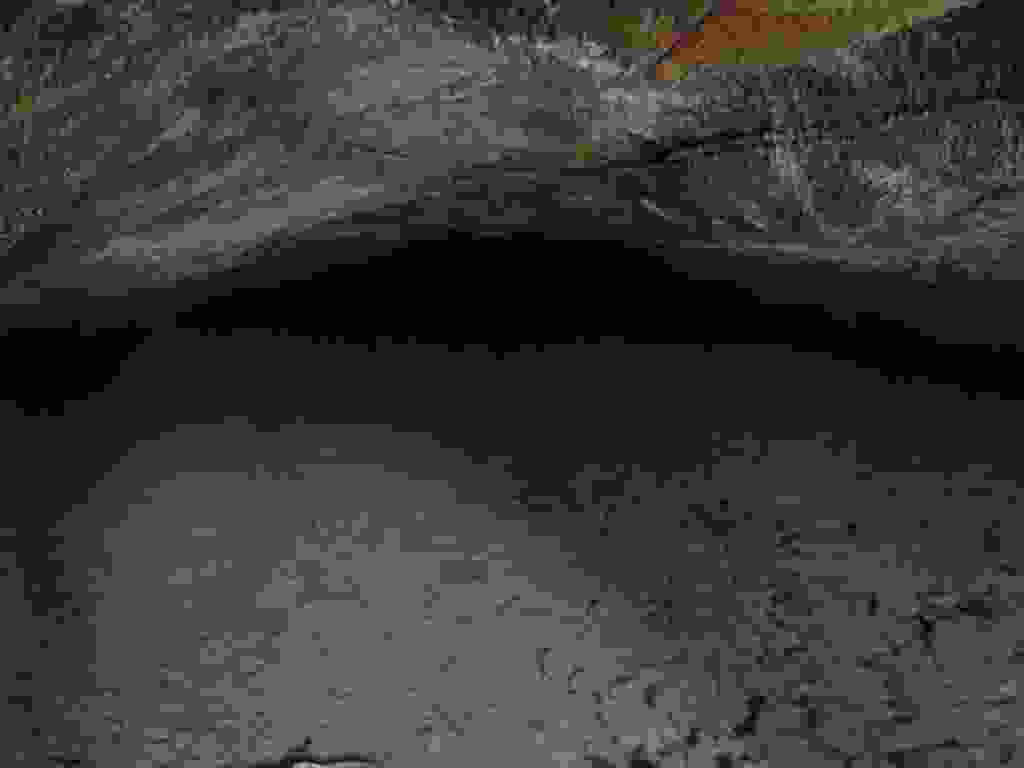
\includegraphics[width=\mywidth]{../wp-content/uploads/2015/07/P7045294-1024x768.jpg} } 
 \newline
 Mirador avec beau point de vue. \newline
 \newline
\centerline{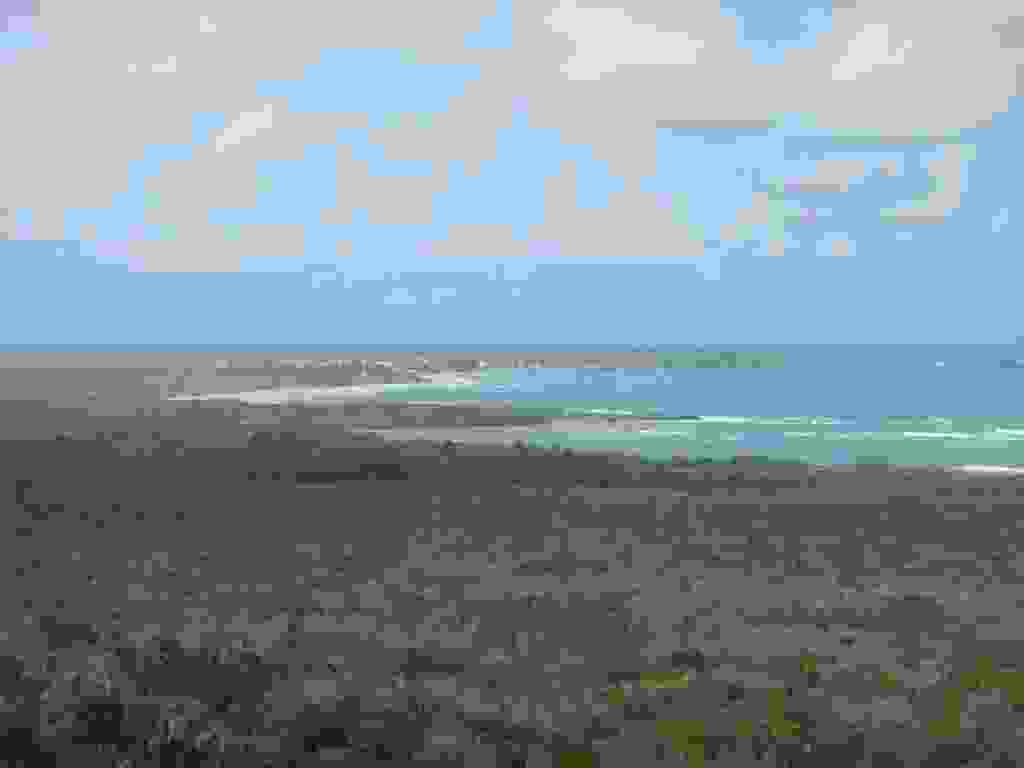
\includegraphics[width=\mywidth]{../wp-content/uploads/2015/07/P7045314-1024x768.jpg} } 
 \newline
 \newline
\centerline{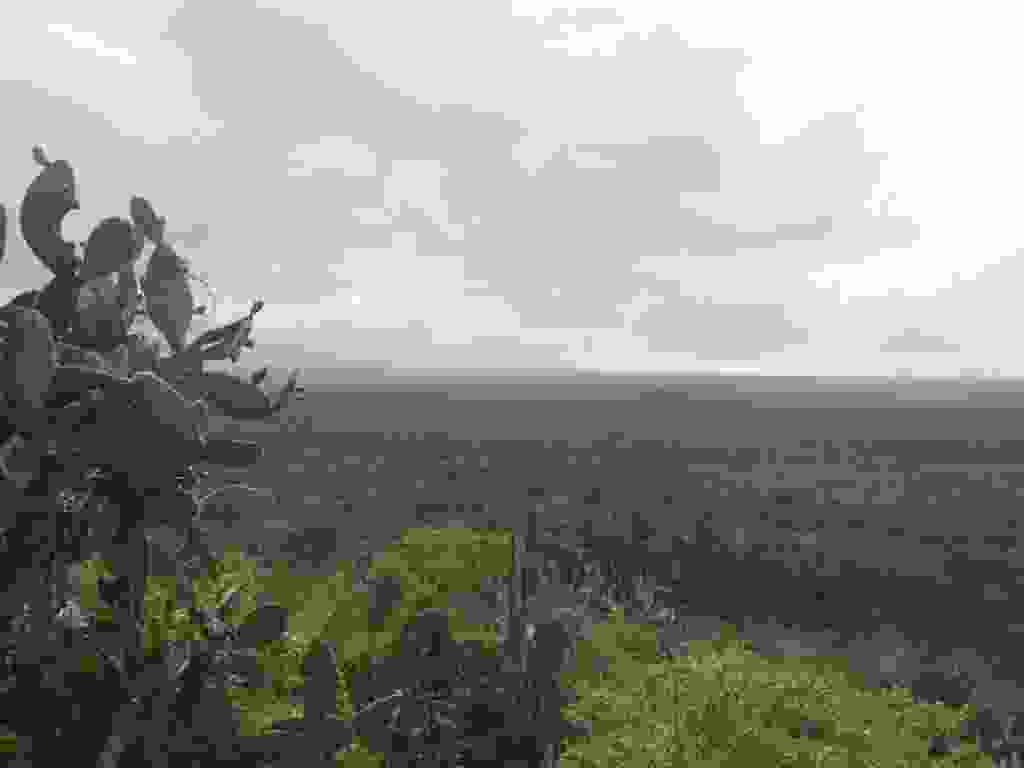
\includegraphics[width=\mywidth]{../wp-content/uploads/2015/07/P7045312-1024x768.jpg} } 
 \newline
 Je finis la journée à Concha de Perla où je croise quelques phoques. \newline
 \newline
\centerline{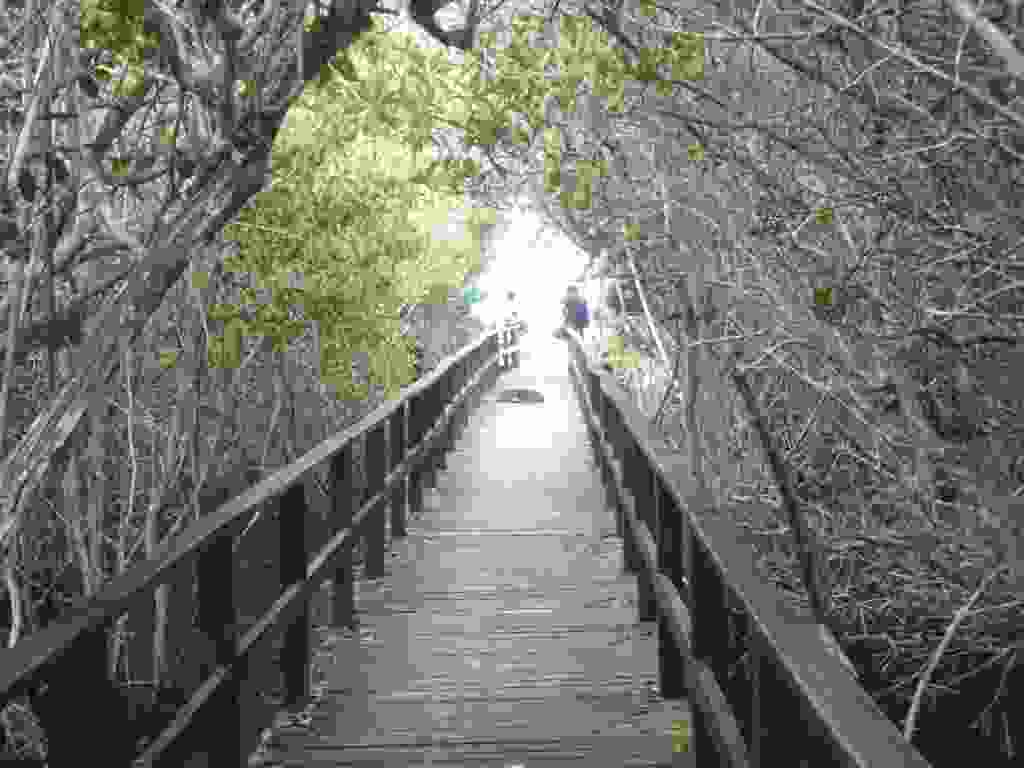
\includegraphics[width=\mywidth]{../wp-content/uploads/2015/07/P7055337-1024x768.jpg} } 
 \newline
 \newline
\centerline{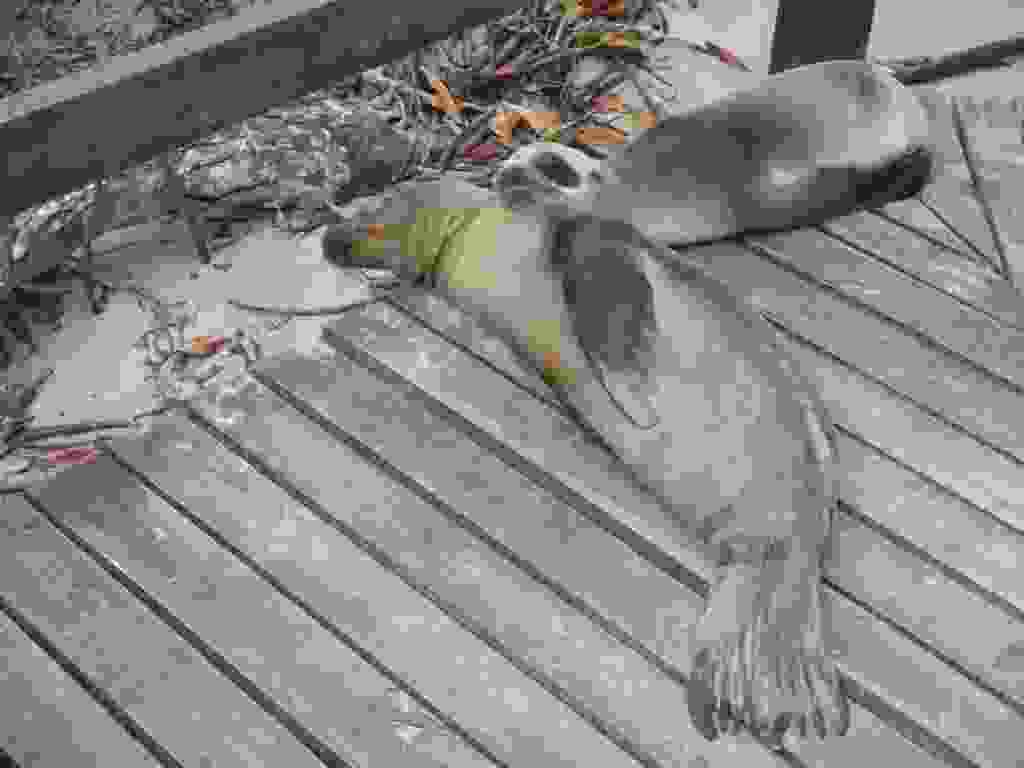
\includegraphics[width=\mywidth]{../wp-content/uploads/2015/07/P7055335-1024x768.jpg} } 
 \newline
 \newline
\centerline{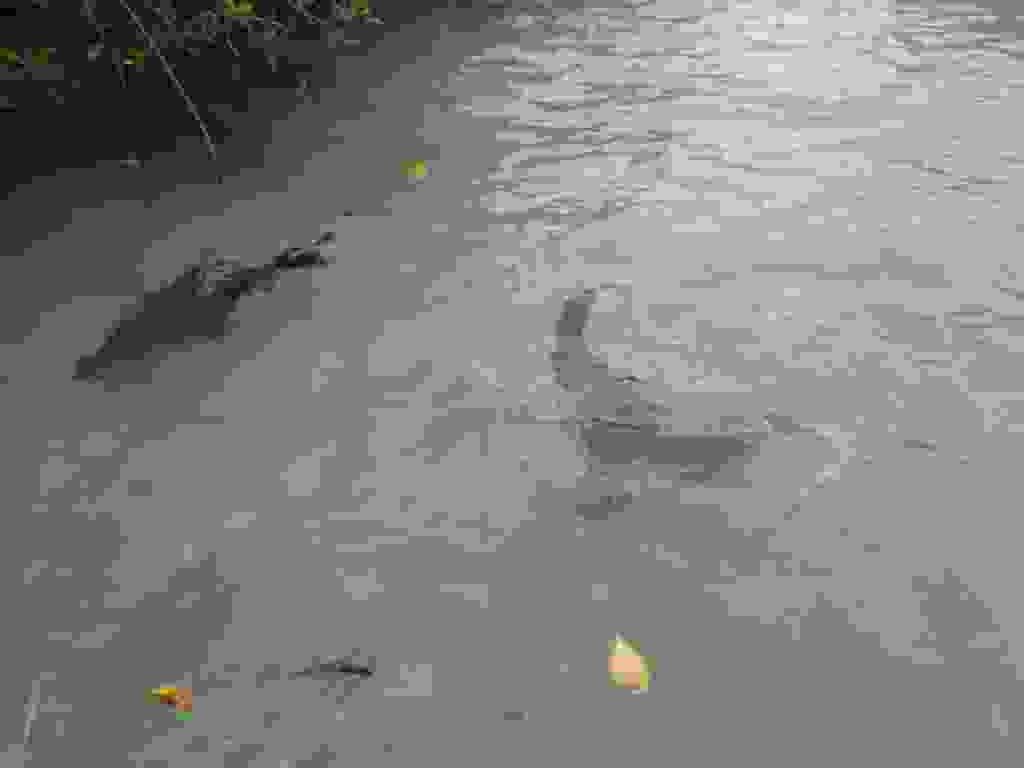
\includegraphics[width=\mywidth]{../wp-content/uploads/2015/07/P7055334-1024x768.jpg} } 
 \newline
 Le lendemain montée au volcan Sierra Negra qui a le 2e plus grand cratère du monde. \newline
 \newline
\centerline{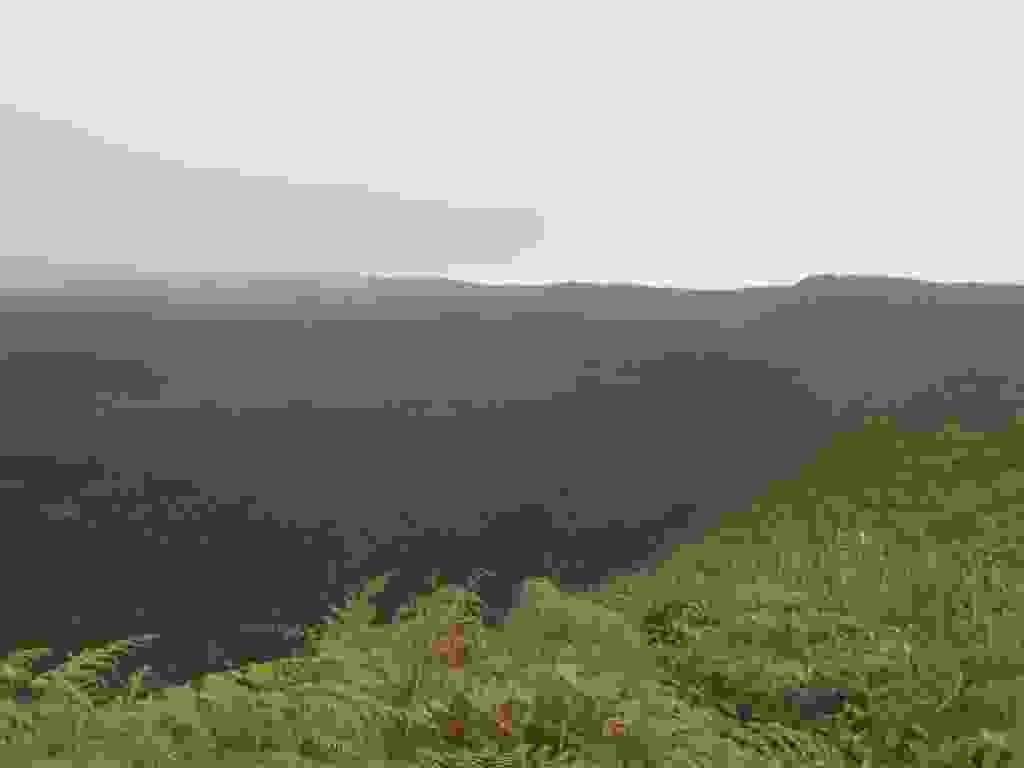
\includegraphics[width=\mywidth]{../wp-content/uploads/2015/07/P7055345-1024x768.jpg} } 
 \newline
 \newline
\centerline{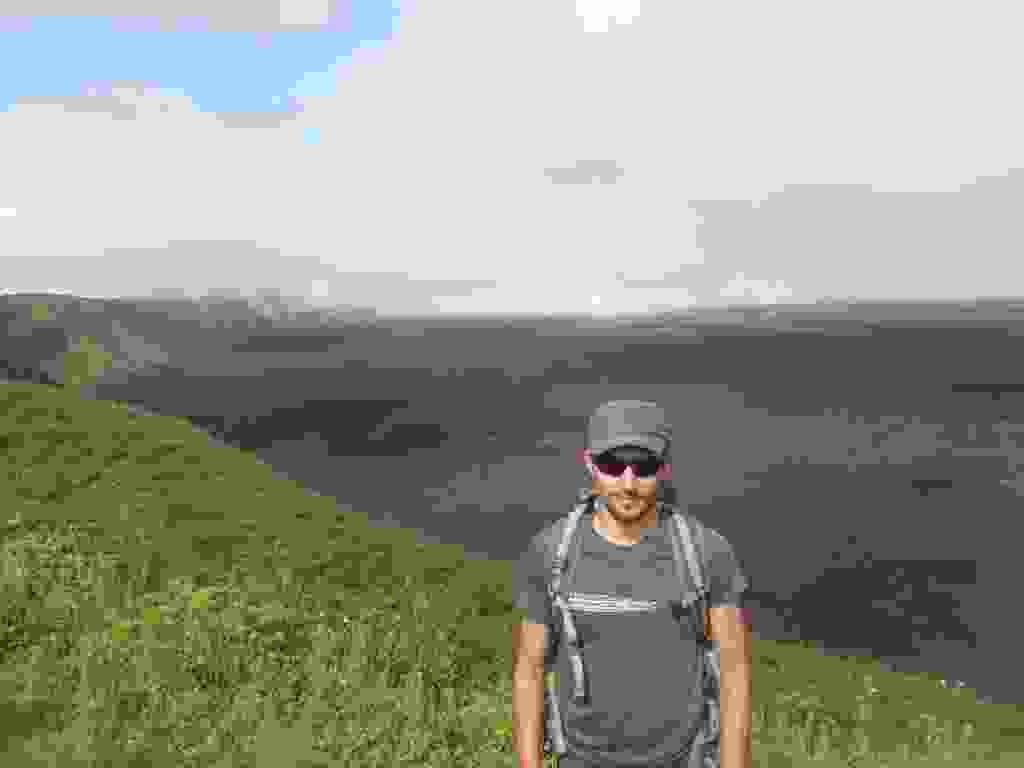
\includegraphics[width=\mywidth]{../wp-content/uploads/2015/07/P7055351-1024x768.jpg} } 
 \newline
 Un peu plus loin le volcan El Chico avec des paysages lunaires. \newline
 \newline
\centerline{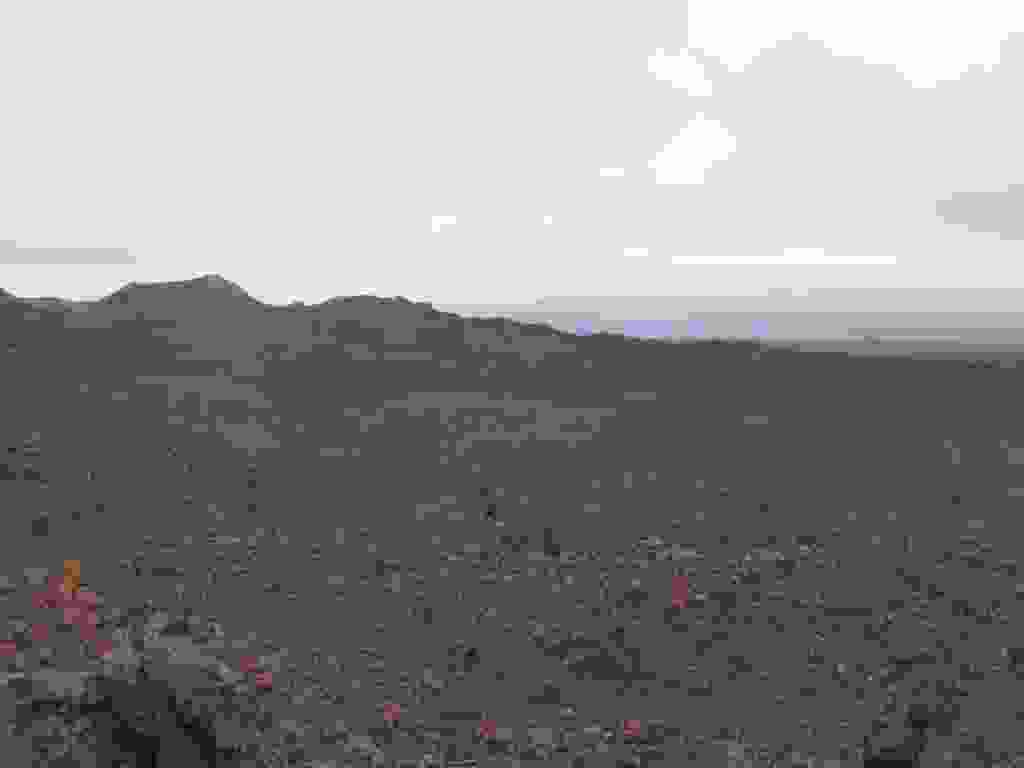
\includegraphics[width=\mywidth]{../wp-content/uploads/2015/07/P7055357-1024x768.jpg} } 
 \newline
 \newline
\centerline{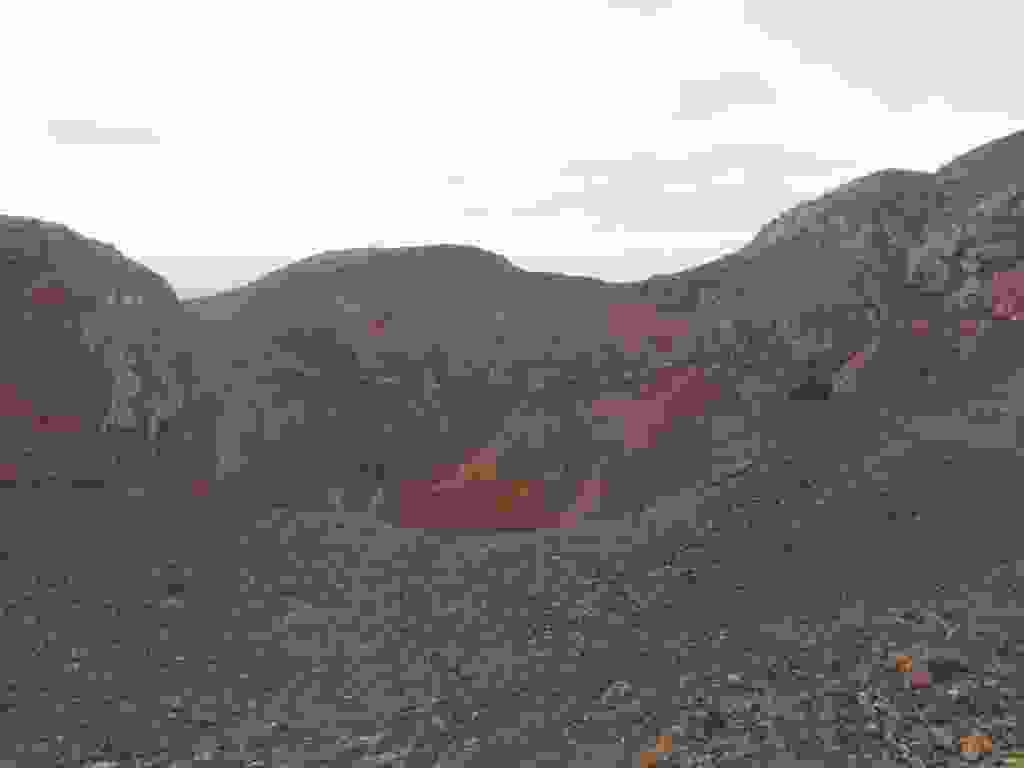
\includegraphics[width=\mywidth]{../wp-content/uploads/2015/07/P7055360-1024x768.jpg} } 
 \newline
 \newline
\centerline{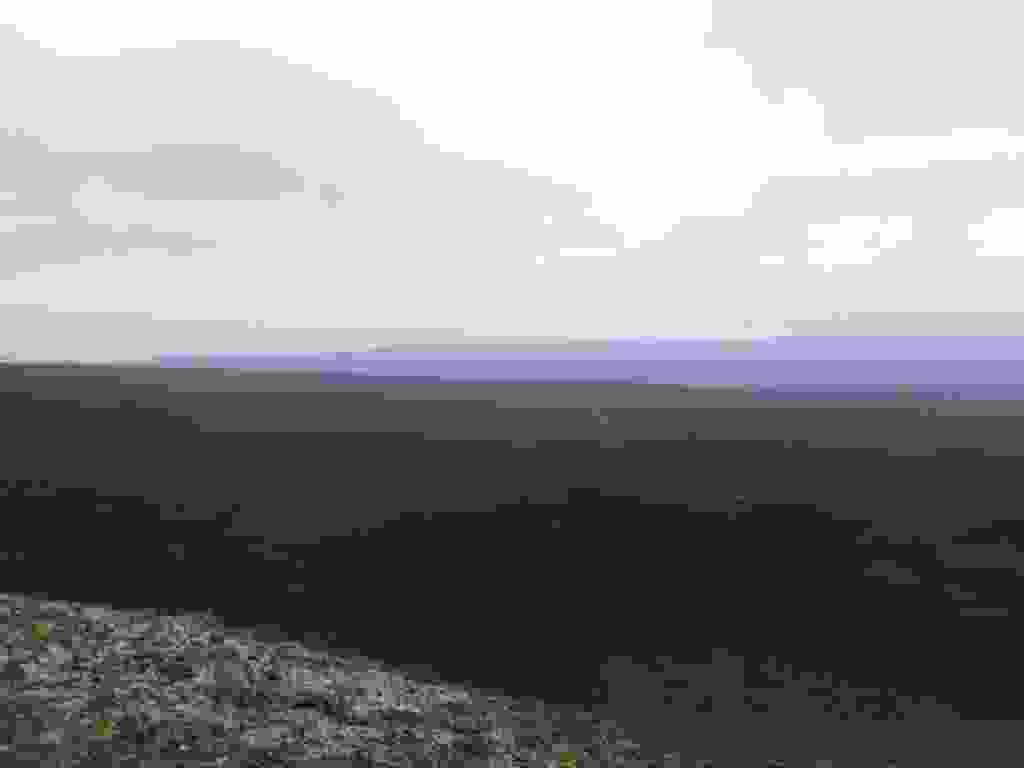
\includegraphics[width=\mywidth]{../wp-content/uploads/2015/07/P7055364-1024x768.jpg} } 
 \newline
 \newline
\centerline{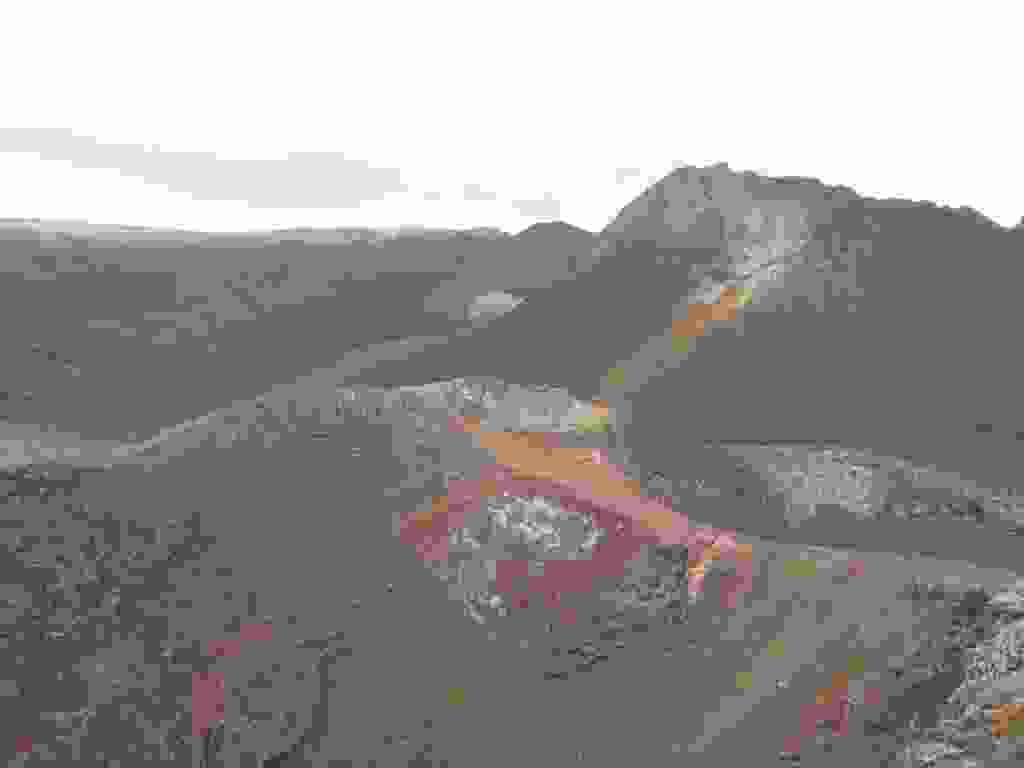
\includegraphics[width=\mywidth]{../wp-content/uploads/2015/07/P7055366-1024x768.jpg} } 
 \newline
 Je fais le tour de snorkelling de Los Tuneles à 1h de bateau de la ville. \newline
 \newline
\centerline{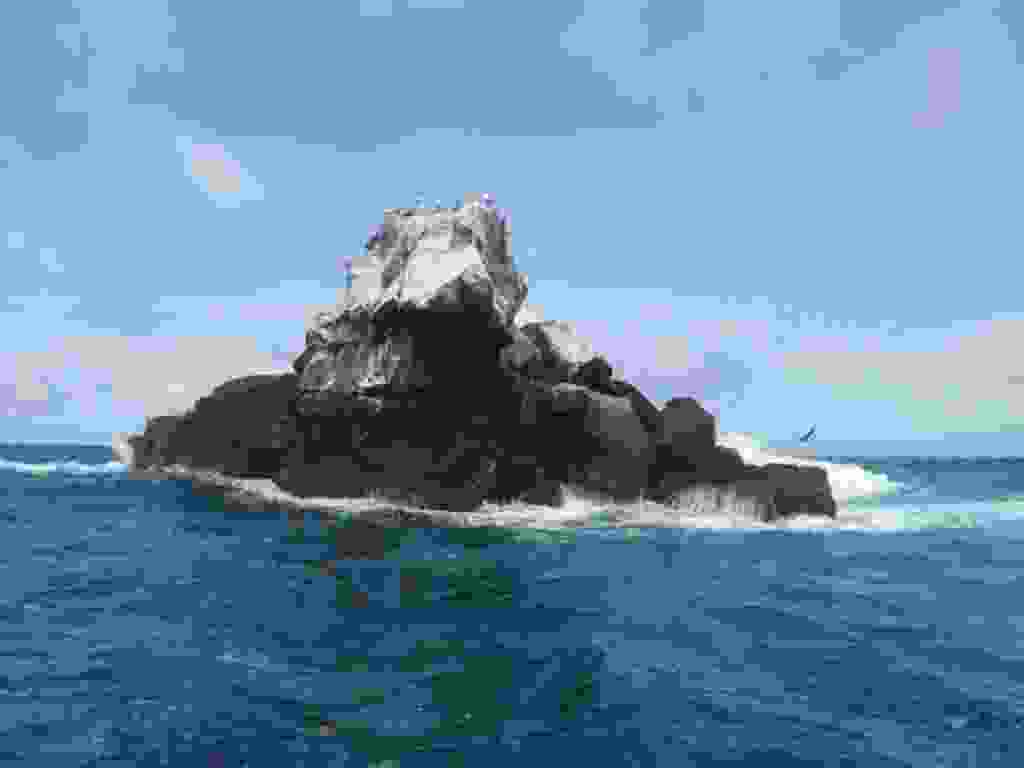
\includegraphics[width=\mywidth]{../wp-content/uploads/2015/07/P7065372-1024x768.jpg} } 
 \newline
 Sur le trajet on descend du bateau pour observer des raies manta : vraiment impressionnantes. \newline
 Les pingouins des Galapagos. \newline
 \newline
\centerline{\includegraphics[width=\mywidth]{../wp-content/uploads/2015/07/P7065376-1024x768.jpg} } 
 \newline
 Puis 2 snorkelling où on peut voir beaucoup de poissons, des tortues marines, des requins (qui dorment), des hippocampes. \newline
 \newline
\centerline{\includegraphics[width=\mywidth]{../wp-content/uploads/2015/07/P7065381-1024x768.jpg} } 
 \newline
 \newline
\centerline{\includegraphics[width=\mywidth]{../wp-content/uploads/2015/07/P7065384-1024x768.jpg} } 
 \newline
 J'ai voulu prendre des photos avec l'appareil étanche : il a pris l'eau et ne marche plus ! Heureusement que c'est arrivé à la fin des Galapagos ! \newline
 Enfin il fallait bien gouter un bon poisson des Galapagos. \newline
 \newline
\centerline{\includegraphics[width=\mywidth]{../wp-content/uploads/2015/07/P7035246-1024x768.jpg} } 
 \newline
 Accompagné d'une biere équatorienne il est bien passé ! \newline
 \newline
\centerline{\includegraphics[width=\mywidth]{../wp-content/uploads/2015/07/P7035244-1024x768.jpg} } 
 \newline

\newpage
 
